 
 % Uses:
 %		SETTINGS.TEX	contains the settings for this document
 %		COMMANDS.TEX	contains commands which can be used while writing
 %		INFO.TEX			contains the author, title and so on for the cover
 %		COVER.TEX			formats the front cover of the document
 %		ABSTRACT.TEX	contains the abstract to be included (if needed)
 %		BIB.BIB				containt the BibTeX entries for the document
 
\documentclass[11pt,a4paper,bibtotoc,idxtotoc,headsepline,footsepline,footexclude,BCOR12mm,DIV13]{scrbook}

% KOMA-Optionen:
%  bibtotoc: include bibliography in table of contents
%  idxtotoc: include index in table of contents
%  headsepline: use horizontalline under heading
%  BCOR: binding correcion (Bindungskorrektur) (e.g.: BCOR5mm)
%  DIV: Number of sheet sections (used for layout) (e.g.: DIV12) 

% include title and author information for the cover
% Set here the title, authors and other stuff to be used for the cover
% This file is used by MAIN.TEX

% set title, authors and stuff for the cover
\def\doctype{Interdisciplinary Project in Finance and Informatics}
\def\title{Leads and Lags of Corporate Bonds and Stocks}
\def\titleGer{Leads und Lags von Unternehmensanleihen und Aktien}
\def\author{Alex Kulikov}
\def\date{March 31, 2021}

% text to appear in the footer
\def\footertext{}

% include settings
% Included by MAIN.TEX
% Defines the settings for the CAMP report document

\renewcommand{\sectfont}{\normalfont \bfseries}        % Schriftart der Kopfzeile

% manipulate footer
\usepackage{scrpage2}
\pagestyle{scrheadings}
\ifoot[\footertext]{\footertext} % \footertext set in INFO.TEX
%\setkomafont{pagehead}{\normalfont\rmfamily}
\setkomafont{pagenumber}{\normalfont\rmfamily}

%% allow sophisticated control structures
\usepackage{ifthen}

% use Palatino as default font
\usepackage{palatino}

% enable special PostScript fonts
\usepackage{pifont}

% make thumbnails
\usepackage{thumbpdf}

%to use the subfigures
\usepackage{subfigure}


\usepackage{colortbl}


%% show program code\ldots
%\usepackage{verbatim}
%\usepackage{program}
\usepackage{minted}
\usepackage{listings}

\usepackage{caption}

% writing pseudo-code
\usepackage{algorithm}
%\usepackage{algorithmic}
\usepackage[noend]{algpseudocode}% http://ctan.org/pkg/algorithmicx
%\usepackage[linesnumbered,ruled]{algorithm2e}

%% enable TUM symbols on title page
\usepackage{styles/tumlogo}


\usepackage{multirow}

%% use colors
\usepackage{color}

%% make fancy math
\usepackage{amsmath}
\usepackage{amsfonts}
\usepackage{amssymb}
\usepackage{textcomp}
\usepackage{yhmath} % f�r die adots 
%% mark text as preliminary
%\usepackage[draft,german,scrtime]{prelim2e}

%% create an index
\usepackage{makeidx}

% for the program environment
\usepackage{float}

%% load german babel package for german abstract
%\usepackage[german,american]{babel}
\usepackage[german,english]{babel}
\selectlanguage{english}

% use german characters as well
\usepackage[latin1]{inputenc}       % allow Latin1 characters

% use initals dropped caps - doesn't work with PDF
\usepackage{styles/dropping}


\usepackage{styles/shortoverview}
%----------------------------------------------------
%      Graphics and Hyperlinks
%----------------------------------------------------

%% check for pdfTeX
\ifx\pdftexversion\undefined
 %% use PostScript graphics
 \usepackage[dvips]{graphicx}
 \DeclareGraphicsExtensions{.eps,.epsi}
 \graphicspath{{figures/}{figures/review}} 
 %% allow rotations
 \usepackage{rotating}
 %% mark pages as draft copies
 %\usepackage[english,all,light]{draftcopy}
 %% use hypertex version of hyperref
 \usepackage[hypertex,hyperindex=false,colorlinks=false]{hyperref}
\else %% reduce output size \pdfcompresslevel=9
 %% declare pdfinfo
 %\pdfinfo { 
 %  /Title (my title) 
 %  /Creator (pdfLaTeX) 
 %  /Author (my name) 
 %  /Subject (my subject	) 
 %  /Keywords (my keywords)
 %}
 %% use pdf or jpg graphics
 \usepackage[pdftex]{graphicx}
 \DeclareGraphicsExtensions{.jpg,.JPG,.png,.pdf,.eps}
 \graphicspath{{figures/}} 
 
 %% Load float package, for enabling floating extensions
 \usepackage{float}
 
 %% allow rotations
 \usepackage{rotating}
 %% use pdftex version of hyperref
 \usepackage[pdftex,colorlinks=true,linkcolor=black,citecolor=black,%
 anchorcolor=black,urlcolor=black,bookmarks=true,%
 bookmarksopen=true,bookmarksopenlevel=0,plainpages=false%
 bookmarksnumbered=true,hyperindex=false,pdfstartview=%
 ]{hyperref}
%
%\usepackage[pdftex,colorlinks=false,linkcolor=red,citecolor=red,%
% anchorcolor=red,urlcolor=red,bookmarks=true,%
% bookmarksopen=true,bookmarksopenlevel=0,plainpages=false%
% bookmarksnumbered=true,hyperindex=false,pdfstartview=%
% ]{hyperref}
\fi




%% Fancy chapters
%\usepackage[Lenny]{fncychap}
%\usepackage[Glenn]{fncychap}
%\usepackage[Bjarne]{fncychap}

%\usepackage[avantgarde]{quotchap}

% set the bibliography style
%\bibliographystyle{styles/bauermaNum}
%\bibliographystyle{alpha}
\bibliographystyle{plain}

% include commands
% Commands to be used within the TUM report document
% Included by MAIN.TEX
% Please include your own cool commands here. 
% Be only sure to comment it sufficiently so others can use it.

%-------------------------------------------------------------
%                      Own Commands
%-------------------------------------------------------------


%-------------------------------------------------------------
% math stuff -------------------------------------------------

% nice R, N, C
\newcommand{\nat}{\mathbb{N}}
\newcommand{\real}{\mathbb{R}}
\newcommand{\compl}{\mathbb{C}}



% norm
\newcommand{\norm}[1]{\left\| #1 \right\|}

% un demi
\newcommand{\half}{\frac{1}{2}}

% parantheses
\newcommand{\parenth}[1]{ \left( #1 \right) }
\newcommand{\bracket}[1]{ \left[ #1 \right] }
\newcommand{\accolade}[1]{ \left\{ #1 \right\} }
%\newcommand{\angle}[1]{ \left\langle  #1 \right\rangle }

% partial derivative: %#1 function, #2 which variable
% simple / single line version
\newcommand{\pardevS}[2]{ \delta_{#1} f(#2) }
% fraction version
\newcommand{\pardevF}[2]{ \frac{\partial #1}{\partial #2} }

% render vectors: 3 and 4 dimensional
\newcommand{\veciii}[3]{\left[ \begin{array}[h]{c} #1 \\ #2 \\ #3	\end{array} \right]}
\newcommand{\veciv}[4]{\left[ \begin{array}[h]{c} #1 \\ #2 \\ #3 \\ #4	\end{array} \right]}

% render matrices: 3  dimensional (arguments in row first order)
\newcommand{\matiii}[9]{\left[ \begin{array}[h]{ccc} #1 & #2 & #3 \\ #4 & #5 & #6 \\ #7 & #8 & #9	\end{array} \right]}
%DOESN'T WORK,DON'T KNOW WHY \newcommand{\mativ}[16]{\left[ \begin{array}[h]{cccc} #1 & #2 & #3 & #4 \\ #5 & #6 & #7 & #8 \\ #9 & #10 & #11 & #12 \\ #13 & #14 & #15 & #16 \end{array} \right]}


%-------------------------------------------------------------
%-------------------------------------------------------------


%-------------------------------------------------------------
% some abreviations ------------------------------------------
\newcommand{\Reg}{$^{\textregistered}$}
\newcommand{\reg}{$^{\textregistered}$ }
\newcommand{\Tm}{\texttrademark}
\newcommand{\tm}{\texttrademark~}
\newcommand {\bsl} {$\backslash$}

%-------------------------------------------------------------
%-------------------------------------------------------------


%-------------------------------------------------------------
% formating --------------------------------------------------

% Theorem & Co environments and counters
\newtheorem{theorem}{Theorem}[chapter]
\newtheorem{lemma}[theorem]{Lemma}
\newtheorem{corollary}[theorem]{Corollary}
\newtheorem{remark}[theorem]{Remark}
\newtheorem{definition}[theorem]{Definition}
\newtheorem{equat}[theorem]{Equation}
\newtheorem{example}[theorem]{Example}
%\newtheorem{algorithm}[theorem]{Algorithm}

% inserting figures
\newcommand{\insertfigure}[4]{ % Filename, Caption, Label, Width percent of textwidth
	\begin{figure}[htbp]
		\begin{center}
			\includegraphics[width=#4\textwidth]{#1}
		\end{center}
		\vspace{-0.4cm}
		\caption{#2}
		\label{#3}
	\end{figure}
}




% referecing figures

\newcommand{\refFigure}[1]{ %label
	figure \ref{#1}
}
\newcommand{\refChapter}[1]{ %label
	chapter \ref{#1}
}

\newcommand{\refSection}[1]{ %label
	section \ref{#1}
}

\newcommand{\refParagraph}[1]{ %label
	paragraph \ref{#1}
}

\newcommand{\refEquation}[1]{ %label
	equation \ref{#1}
}

\newcommand{\refTable}[1]{ %label
	table \ref{#1}
}




\newcommand{\rigidTransform}[2]
{
	${}^{#2}\!\mathbf{H}_{#1}$
}

%code, in typewriter
\newcommand{\code}[1]
 {\texttt{#1}}

% comment that appears on the border - very practical !!!
\newcommand{\comment}[1]{\marginpar{\raggedright \noindent \footnotesize {\sl #1} }}

% page clearing
\newcommand{\clearemptydoublepage}{%
  \ifthenelse{\boolean{@twoside}}{\newpage{\pagestyle{empty}\cleardoublepage}}%
  {\clearpage}}


%-------------------------------------------------------------
%-------------------------------------------------------------


\newcommand{\etAl}{\emph{et al.}\mbox{ }}

\makeglossary

\begin{document}
	
	% New definitions
	\algnewcommand\algorithmicswitch{\textbf{switch}}
	\algnewcommand\algorithmiccase{\textbf{case}}
	\algnewcommand\algorithmicassert{\texttt{assert}}
	\algnewcommand\Assert[1]{\State \algorithmicassert(#1)}%
	% switch case
	\algdef{SE}[SWITCH]{Switch}{EndSwitch}[1]{\algorithmicswitch\ #1\ \algorithmicdo}{\algorithmicend\ \algorithmicswitch}%
	\algdef{SE}[CASE]{Case}{EndCase}[1]{\algorithmiccase\ #1}{\algorithmicend\ \algorithmiccase}%
	\algtext*{EndSwitch}%
	\algtext*{EndCase}%
	

	\frontmatter		
		%% The front cover for the TUM report document.
% Included by MAIN.TEX


%--------------------------------------------------
% The Front Cover
%--------------------------------------------------

% The front cover for the TUM document.
% Included by MAIN.TEX


%--------------------------------------------------
% The Front Cover
%--------------------------------------------------

% correct BCOR - undo at the end !!!
\def\bcorcor{0.15cm}
\addtolength{\hoffset}{\bcorcor}

\thispagestyle{empty}

 \vspace{4cm}
\begin{center}
	       \oTUM{4cm}
	   
	   \vspace{5mm}     
	   \huge DEPARTMENT OF INFORMATICS\\ 
	   \vspace{0.5cm}
	 \large TECHNICAL UNIVERSITY OF MUNICH\\
    \vspace{1mm}
        
	\end{center}
		

\vspace{15mm}
\begin{center}

   {\Large \doctype}

  \vspace{20mm}
  
  {\huge\bf \title}\\%[3ex]
  
  
  \vspace{15mm}
  
  
  {\LARGE  \author}
  
  \vspace{10mm}
  
  \begin{figure}[h!]
  \centering
   
\includegraphics[width=4cm]{styles/informat.png}
  \end{figure}
  
  \end{center}		
		%\clearemptydoublepage	
		%% The titlepage for the CAMP report document.
% Included by MAIN.TEX


%--------------------------------------------------
% The title page
%--------------------------------------------------

% correct BCOR - undo at the end !!!
\def\bcorcor{0.15cm}
\addtolength{\hoffset}{\bcorcor}

\thispagestyle{empty}

 \vspace{10mm}
\begin{center}
	       \oTUM{4cm}
	   
	   \vspace{5mm}     
	   \huge DEPARTMENT OF FINANCE\\ 
	   \vspace{0.5cm}
	 \large TECHNICAL UNIVERSITY OF MUNICH\\
        
	\end{center}
		

\vspace{10mm}
\begin{center}

   {\Large \doctype}

  \vspace{10mm}
  
  {\LARGE \title}\\
  
  
  \vspace{10mm}
  
  
  {\LARGE  \titleGer}\\
  
  
  \vspace{10mm}

    %\hfill
    \begin{tabular}{ll}
	   \Large Author:     & \Large \author \\[2mm]
	   \Large Supervisor:    & \Large Prof. Dr. Sebastian M\"{u}ller \\[2mm]				
	   \Large Advisor:	& \Large Zihan Gong \\[2mm]
	   \Large Date:       & \Large March 31, 2021
	 \end{tabular}
	 
	 \vspace{5mm}
	 
	 \begin{figure}[h!]
  \centering
   
\includegraphics[width=4cm]{styles/informat.png}
  \end{figure}
   

\end{center}

% undo BCOR correction
\addtolength{\hoffset}{\bcorcor}	
		%\input{components/cover_maschmeyer}	
		%\clearemptydoublepage			
		% The titlepage for the CAMP report document.
% Included by MAIN.TEX


%--------------------------------------------------
% The title page
%--------------------------------------------------

% correct BCOR - undo at the end !!!
\def\bcorcor{0.15cm}
\addtolength{\hoffset}{\bcorcor}

\thispagestyle{empty}

 \vspace{10mm}
\begin{center}
	       \oTUM{4cm}
	   
	   \vspace{5mm}     
	   \huge DEPARTMENT OF FINANCE\\ 
	   \vspace{0.5cm}
	 \large TECHNICAL UNIVERSITY OF MUNICH\\
        
	\end{center}
		

\vspace{10mm}
\begin{center}

   {\Large \doctype}

  \vspace{10mm}
  
  {\LARGE \title}\\
  
  
  \vspace{10mm}
  
  
  {\LARGE  \titleGer}\\
  
  
  \vspace{10mm}

    %\hfill
    \begin{tabular}{ll}
	   \Large Author:     & \Large \author \\[2mm]
	   \Large Supervisor:    & \Large Prof. Dr. Sebastian M\"{u}ller \\[2mm]				
	   \Large Advisor:	& \Large Zihan Gong \\[2mm]
	   \Large Date:       & \Large March 31, 2021
	 \end{tabular}
	 
	 \vspace{5mm}
	 
	 \begin{figure}[h!]
  \centering
   
\includegraphics[width=4cm]{styles/informat.png}
  \end{figure}
   

\end{center}

% undo BCOR correction
\addtolength{\hoffset}{\bcorcor}	
		%%\thispagestyle{empty}
\selectlanguage{english}
	%\vspace*{0.8\textheight}
	%\noindent
	I confirm that this documentation as part of my interdisciplinary project is my own work and I have documented all sources and material used.
	
	%\vspace{15mm}
	%\noindent
	%Munich, \today \hspace{5cm} \author
\selectlanguage{english}	
		%\clearemptydoublepage
\phantomsection
\addcontentsline{toc}{chapter}{Acknowledgements}	


%\chapter*{Acknowledgements}

\vspace*{2cm}

\begin{center}
{\Large \bf Acknowledgments}
\end{center}

\vspace{1cm}




	
		% Abstract for the TUM report document
% Included by MAIN.TEX

\phantomsection
\addcontentsline{toc}{chapter}{Abstract}	

\vspace*{2cm}
\begin{center}
{\Large \bf Abstract}
\end{center}
\vspace{1cm}

In the scope of an Interdisciplinary Project at the Technical University of Munich, an international, extendable corporate bonds database had to be built up from scratch for further empirical research. For this purpose, an automatic extraction tool for financial securities data has been developed on top of the interface provided by the Refinitiv Datastream financial database. The required static and time series corporate bond data -- consisting of over 60.000 bonds -- has been downloaded, cleaned, and prepared for further research. Additionally, a matching algorithm has been developed to join corporate bond and stock data with each other based on their issuing company. The algorithm utilizes fuzzy string matching based on company name as well as key-based matching based on the CUSIP-9 parameter, and has shown a matching ratio of around 45\% without a globally unique company identifier. Further, the distribution of corporate bond returns has been found in-line with expectations, which served as a sanity check for the downloaded data. Finally, correlation and regression analyses have shown stock data to be more efficient in incorporating new information than corporate bond data based on a 1-month lead. 

		%% German abstract for the CAMP report document
% Included by MAIN.TEX


\clearemptydoublepage






\vspace*{2cm}
\begin{center}
{\Large \bf Zusammenfassung}
\end{center}
\vspace{1cm}

Die vorliegende Arbeit befasst sich mit der Anpassung und Parallelisierung effizienter Skyline Algorithmen f�r moderne Hauptspeicher-Datenbanksysteme. Au�erdem richtet sie den ART Baum f�r kategorische Skyline Berechnung ein. 

Um Datenbank-Anfragen schneller bearbeiten zu k�nnen, werden einige der bekannten Skyline Algorithmen so angepasst, dass sie als Baustein direkt in eine Hauptspeicher-Datenbank aufgenommen werden k�nnen. Daraufhin werden moderne Parallelisierungstechniken vorgestellt und auf die Skyline Algorithmen angewendet. Die gemessenen Performanzergebnisse bezeugen, dass die vorgeschlagenen Parallelisierungsans�tze die Laufzeit der Algorithmen in parallelisierter Umgebung verbessern konnten. 

Dar�ber hinaus wurde der ART Baum dazu verwendet, den neuartigen Algorithmus SARTS zu entwerfen. Der Algorithmus eignet sich besonders gut zur progressiven Berechnung der Skyline in Online-Umgebungen. Im Rahmen der durchgef�hrten Tests zeigt der Algorithmus sehr solide Laufzeiten auch bei gr��eren Tupelmengen und verbraucht dabei bis zu 20-mal weniger Speicher als sein direkter Vorg�nger ST-S. %Letzteres verdankt er dem effizienten Speicherumgang des ART Baums. 

%Mit steigender Nachfrage nach interaktiven Services im Internet w�chst auch der Bedarf nach effizienten Algorithmen, welche sich mit der Verarbeitung der entstehenden Datenmengen befassen. Eine der heutzutage immer h�ufiger eingesetzten Methoden zur Filterung der Datenbasis ist die Berechnung der Skyline einer Menge von Tupeln. Zu der Skyline geh�ren diejenigen Tupel, welche interessant f�r den Anfragesteller sind. Ein Tupel gilt als interessant, sofern es von keinem anderen Tupel aus der Datenmenge dominiert wird. 



		\tableofcontents
		%\clearemptydoublepage

\phantomsection
%\addcontentsline{toc}{chapter}{Outline of the Thesis}

%\begin{center}
%	\huge{Outline of the Thesis}
%\end{center}
%
%
%
%
%%--------------------------------------------------------------------
%\section*{Part I: Introduction and Theory}
%
%\noindent {\scshape Chapter 1: Introduction}  \vspace{1mm}
%
%\noindent  This chapter presents an overview of the thesis and it purpose. Furthermore, it will discuss the sense of life in a very general approach.  \\
%
%\noindent {\scshape Chapter 2: Theory}  \vspace{1mm}
%
%\noindent  No thesis without theory.   \\
%
%%--------------------------------------------------------------------
%\section*{Part II: The Real Work}
%
%\noindent {\scshape Chapter 3: Overview}  \vspace{1mm}
%
%\noindent  This chapter presents the requirements for the process.

	\mainmatter	
%		\part[Introduction and Theory]{Introduction and Theory}
%		\label{part:introAndBackgroundTheory}

		\chapter{Introduction} \label{chapter:Introduction}
In the scope of an Interdisciplinary Project (\textit{IDP} in the following) at the Technical University of Munich, the lead and lag relationship between corporate bond and stock returns has to be analyzed. With the needed stock data already provided, the first step of the IDP is to develop a tool which would be able to automatically extract static and time series data from the Thomson Reuters Datastream financial database. In the second step of the IDP, the extracted bond data has to be cleaned and prepared for further analysis by various transformation techniques. Additionally, a matching approach to join the stock and bond datasets by issuing company needs to be developed. In the third and final step of the IDP, the resulting bond-stock database has to be checked for any sort of lead and/or lag relationships within bond and stock return pairs. 

The extracted corporate bond data, both static and time series, has a wide array of applications, ranging from descriptive historical applications to predictive models, and will thus be of significant value for future financial research. In order to make use of the most recent market trends and developments, the acquired bond database, as well as the existing stock information, should be extendable, such that recent data can be accumulated in a continuous manner. This is where the tool for automated data extraction from Refinitiv Datastream comes into play. It has to provide capabilities to download financial securities data in a convenient and seamless manner, as far as technology allows. Since corporate bonds and their qualities as an investment instrument are often compared to equities \cite{asset-management}, it only makes sense to additionally develop an efficient approach to analyze the two asset classes "side-by-side". At this point, a suitable matching mechanism to join bond and equity data by their issuing company is of paramount importance, and can be used in many different analysis scenarios. At the end of any financial analysis, researchers are always interested in the insights into the functioning of financial markets and the optimal investment thesis which arises therefrom. Analyzing the lead and lag relationship of corporate stocks and bonds can provide such an investment thesis based on the efficiency with which the two asset classes incorporate new information in their pricing \cite{lead-lag-source}. From a practical perspective, if I, as an investor, knew that today's stock returns predict bond returns in the next month, I could allocate my assets accordingly to gain a higher-than-usual profit from my investment. While the constraints and influence of market equilibrium conditions on such an investment strategy could be analyzed separately \cite{asset-management}, the gain of such knowledge is undoubtedly of significant academical and practical importance. 



		\chapter{Datastream Extraction Tool} \label{chapter:datastream-extraction-tool}
In order to draw any conclusions regarding the relationship of bond and stock returns, the respective static and time series data needs to be acquired first. Since equity data is already available from the beginning of the IDP, the bond data is the only one which had to be acquired. For bond data extraction, the financial database product Datastream, provided by Thomson Reuters, can be used, since it is licensed for usage by TUM students and employees. 

\section{Download Solution} \label{section:download-solution}
As Thomson Reuters has a wide range of products which can be used for different types of data, the first thing that needed to be done, was to determine the most suitable product to download both static and time series data for corporate bonds. After some time spent reading up and gathering information on the Thomson Reuters product portfolio, it became apparent that some of the products, such as the TR Python API, are only suitable for equity data download, and not for corporate bonds, and only have a very limited number of parameters available for download. On the other hand, it was found that other Thomson Reuters products, which would normally be suitable for automated download of bond data, such as e.g. DataScope Select (DSS) or Thomson Reuters Tick History (TRTH), are not included in the existing academic license. Other products -- noticeably the Datastream Web Service (DSWS) API, which is most suited for such requests -- are generally not available for academic clients. 

These findings were a significant setback for the bond data extraction, since the only option left to acquire large amounts of corporate bond data, was over the Datastream Add-In for Microsoft Excel. While this add-in is rather convenient for small-scale manual requests with the help of so-called request tables, it is not optimized for large data extraction queries. It does not provide an API for customizable requests. Instead, communication with the Datastream server is handled over a single API call available in VBA. This one and only callable function is implemented in C++, and can only be invoked in a black-box manner, since the provider does not give out its implementation. This leads to only one possible solution to automatically extract corporate bond data from Datastream. It can be described with the following steps: 
\begin{enumerate}
		\item Acquire Datastream codes / identifiers for all financial instruments which need to be downloaded.
		\item Split these identifiers into batches small enough to be processed in a single Datastream request.
		\item Fill a request table with as many requests as needed to include all the batches. 
		\item Launch the Datastream requests for all the batches one after the other. 
		\item Monitor the download process to ensure that the data is being consistently downloaded. 
\end{enumerate}
The programmatic development of the download tool will be based exactly on these five steps. The last step (monitoring the execution) is especially crucial and complex to implement. The reason for this is, as previously mentioned, that the Datastream Excel Add-In is not well-fit for large data downloads. Therefore, the following problems continuously arise during the download process: 
\begin{itemize}
	\item Datastream add-in eventually signs out for no obvious reason. 
	\item Data download hangs, without any notification stating the reason or the hanging fact itself. 
	\item Excel suspends the add-in and places it into a blacklist for repeated faulty behavior. 
\end{itemize}
Since VBA is single threaded and cannot detect or react to erroneous behavior when the download is running, it is impossible to do the monitoring in the VBA/Excel environment. For this purpose, a Python wrapper was developed as will be explained in .%TODO cite

\section{Bond Identifiers Acquisition} \label{section:bond-identifiers-acquisition}
Since for both static and time series requests Datastream requires unique financial instrument codes to be provided, it is first necessary to obtain a list of identifiers for the securities for which the data needs to be downloaded. The most commonly used unique security identifier in Datastream is the so-called Datastream Code (short \textit{dscd}). In the scope of the project two different approaches have been developed for this task, and will be introduced in the following. 

\subsection{Programmatic Identifier Extraction}
For the purpose of this work, we are interested in corporate bonds from all possible jurisdictions, and with any possible coupon an currency parameters. The only restriction is that we only concentrate on the issue date range between Dec 31, 1999 and June 30, 2020 (date of extraction). 

Datastream allows to filter its financial security dataset by these parameters, e.g. when clicking on \textit{Find Series} in a request table. After the securities have been filtered for the desired corporate bonds, these can be selected by repeatedly checking the box to select all bonds on the current page, and then clicking on \textit{Next} to switch to next page. This is due to Datastream not providing an option to select all filtered securities at once if there are more than 4,000. Hence, if there are for instance 60,000 corporate bonds in the database in total, one would not be able to select them all at once. Instead, one would have to select the 15 bonds on the current page and then switch to next page $60,000 / 15 = 4,000$ times. This is of course very cumbersome for the user, and the repeated clicking sounds like a good process to automate programmatically. 

There are multiple tools and scripting languages which enable fast and easy click automation. Specifically for this project I decided to go with Python 3 for this purpose, since it was already part of the environment. One of the packages which enable GUI automation in Python is \textit{pyautogui}. %TODO ref
With build-in methods like $click()$ and $hotkey()$ it enables the user to simulate mouse clicks on the computer screen by giving the functions the screen coordinates of the buttons. Placing the commands into a loop in the right order makes it possible to simulate the entire process of selecting corporate bonds in Datastream. For a possible Python implementation see %TODO
Note that the screen coordinates can significantly differ depending on the screen resolution and window settings. 

While the described approach solves the problem of selecting all the needed corporate bonds from Datastream, there are two downsides to it. The first one is that it is cumbersome for the developer to determine and to enter the screen coordinates of all the buttons involved. The second is that, even when fully automated, the tool needs a lot of time to select and return all of the chosen securities if there are many of them. At this point, the second approach, even though it is manual, is both faster and easier to apply. 

\subsection{Manual Identifier Extraction}
To extract the needed corporate bond identifiers manually, we can make use of the fact that Datastream allows to select all filtered securities at once when there are less than 4,000. Because of this, we can simply split our entire data into multiple chunks that are all smaller than 4,000 bonds in total. This can be done by selecting one or more parameters (the number depends on the size of the dataset) according to which the bonds can be filtered even further. For example, an entire bond dataset with 60,000 bonds in total can be split by coupon size first, and then additionally by currency to produce bond batches of maximum 4,000 bonds each. For a visualization of this approach, see Fig. %TODO create figure
If the split has been done properly, it will include all of the desired securities, since each bond belongs to one particular coupon size as well as currency group. In most cases, there will be only few groups that need to be extracted from the interface. In the case of 60,000 bonds, one would only have $60,000 / 4,000 = 15$ groups in total. In reality, for this concrete use case, 19 different bond groups had to be created. This is because not all splits are perfect, and some of them just consist of 3,500 bonds instead of 4,000 for example. After the splitting work has been done, the resulting bond groups can be extracted manually with just a few clicks. 

\section{Automating the Request Table} \label{section:automating-request-table}
After the bond identifiers in form of \textit{dscd} codes have been extracted, they can be used to retrieve both static and time series data from Datastream. For this purpose, I wrote a VBA program which fully automates the download process. The only input needed from the user is the \textit{dscd }identifiers, the desired variable codes (such as price, issued volume, etc.) as well as the desired time frames in the case of a time series request. Since the program code is rather complex, I will only cover the main approach briefly. A more in-depth description can be found in the appendix to this work. %TODO create appendix

At the beginning, the VBA tool retrieves the user-provided identifiers and datatypes from the respective Excel files. Then, based on the input size, multiple calculations take place. For static information requests not much needs to be done, since these are usually relatively small and only depend on the number of securities for which the data is requested. For time series requests though, the tool estimates how large the entire request will get, depending on dates window, frequency of time points (e.g. daily or quarterly), the number of datatypes, and the number of identifiers. If the request is too large to be processed by Datastream in one run, it gets split into multiple smaller requests of equal size. Since there is no particular metric to estimate in advance whether a particular request will be executed by Datastream, or whether it is too large for that, the tool only computes an approximation based on an empirically measured \textit{Bytes per Field} metric. The single requests then get entered into the request table one below the other, and each receive an own Excel file as destination to store the data. 

As soon as the request table has been filled (which does not take long), the command to process the first request is issued to Datastream. This happens via a call to the single available function, which tells Datastream to process the current request table in a black-box manner. After the request ends, the tool checks whether the requested data has arrived to the destination file. If not, it checks the connection of the Datastream add-in and issues a warning to the user if the add-in unexpectedly disconnected. In both cases, the result of the request is logged, in order for the user to be able to read up on the proceedings later. To prevent the computer from sleeping or going in idle mode, the tool moves the computer mouse pointer after each request with a dedicated VBA function. When the first request of the request table has been processed, the other ones get executed in the same manner one after the other. Note that while it is possible to submit the execution for all requests at once, it is not advisable, since Datastream might issue an error due to the data being too large, or might otherwise simply hang during execution. This is exactly the reason why we had to split up the original request in multiple parts in the first place. 

While the entire Datastream Extraction Tool is much more complex than what has been described here, the given explanation covers the most crucial parts of the download process. At this point, note that the error monitoring step, which was previously mentioned as essential, cannot be completed in VBA due to its single-threaded execution engine. The next section will cover the required workaround for this functionality. 

\section{Error Monitor} \label{section:error-monitor}
In order to provide an error monitoring capacity as well as a graphical user interface (see section \ref{section:user-interface}) for the created VBA tool, a Python 3 wrapper program has been created. For the architecture of the Python-side controller see Fig. \ref{fig:ds-extraction-tool-architecture}. 

\begin{figure}[h]
	\centering
	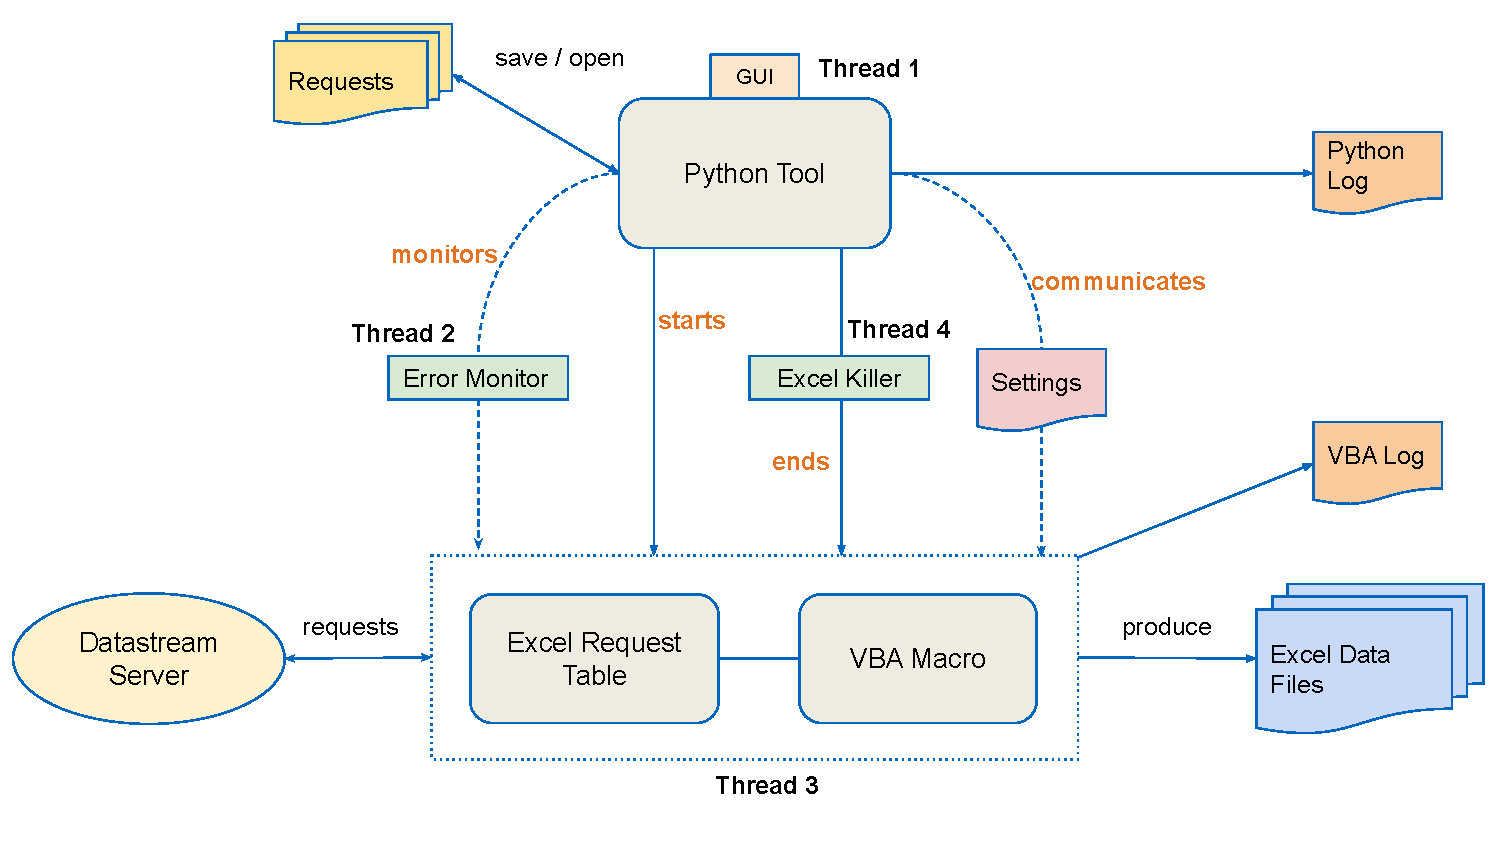
\includegraphics[width=1.1\linewidth]{figures/ds-extraction-tool-architecture}
	\caption{Architecture of the Datastream Extraction Tool}
	\label{fig:ds-extraction-tool-architecture}
\end{figure}



\section{User Interface} \label{section:user-interface}




		\chapter{Data Preparation}  \label{chapter:data-preparation}
As it is often the case with data science projects, the data preparation part is rather tedious. After the static and time series bond data has been extracted from Datastream -- which will likely take several days -- it is available in form of multiple data parts in Excel format. Since it is more convenient to perform further statistical analysis in a dedicated statistical environment, such as Stata or MatLab, the data needs to be brought into 'long' format, and additionally to be cleaned from null entries and outliers. The undertaken procedures are described in the following. 

\section{Data Formatting}  \label{section:data-formatting}
For the static bond data, there is not much to be done in terms of formatting. Its original format, as downloaded from Datastream, is mostly suitable for further analysis and can be directly imported into Stata. 

The downloaded time series data is initially in 'wide' format and has multiple bonds in one row. It looks like shown in Fig. \ref{fig:original-excel-ts-data}. 

\begin{figure}[h]
	\centering
	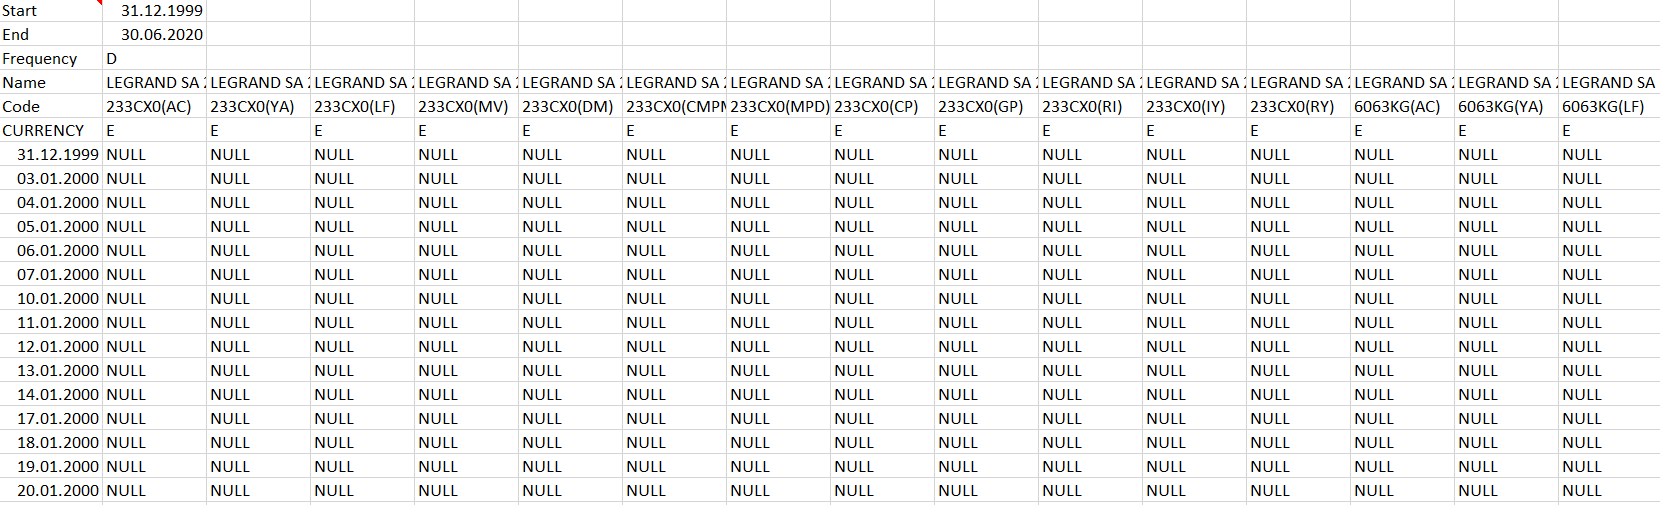
\includegraphics[width=1.0\linewidth]{figures/original-excel-ts-data}
	\caption{Sample of downloaded raw time series bond data}
	\label{fig:original-excel-ts-data}
\end{figure}

The goal is to transform this time series data into 'long' format, as can be seen in Fig. \ref{fig:long-format-excel-ts-data}, by saving the bonds one below the other. 
\begin{figure}[h]
	\centering
	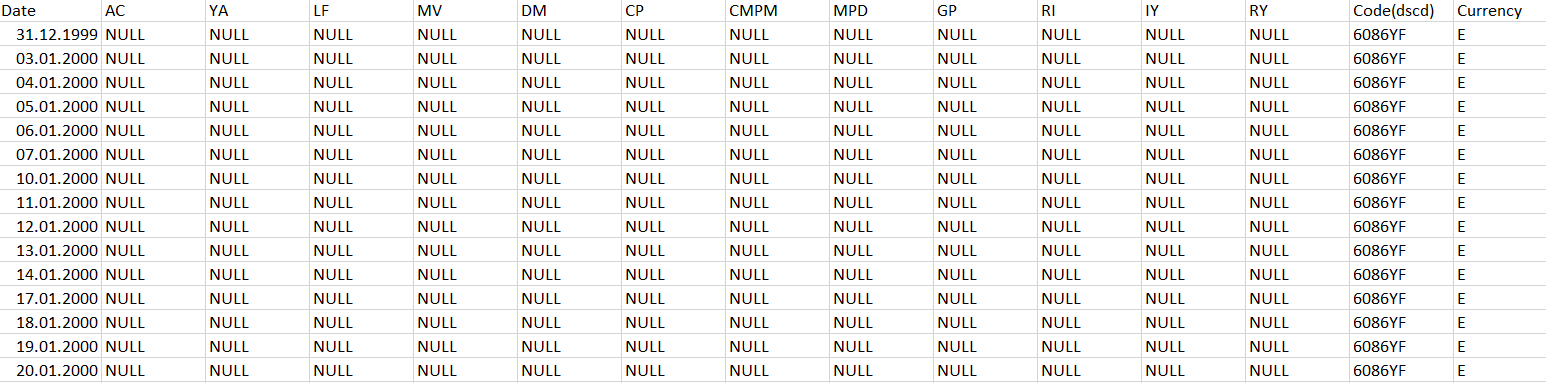
\includegraphics[width=1.0\linewidth]{figures/long-format-excel-ts-data}
	\caption{Sample of downloaded time series bond data in 'long' format}
	\label{fig:long-format-excel-ts-data}
\end{figure}
Additionally, the header has to be removed, and the \textit{dscd} identifier of each bond as well as its currency have to be entered as a separate column for each date instead of being at the top. 

I wrote a VBA macro with a function called \textit{ToLongFormat()} which accomplishes the described task. While Stata might have also been able to do the formatting, I decided to work with VBA at this point, since it is native to the MS Excel environment. While the entire code can be found in the appendix, %TODO Can it?
the main procedure is as follows: 
\begin{enumerate}
	\item Define data layout constants depending on the initial format: header height, number of time stamps, number of datatypes, bonds per block, and number of blocks. A block is defined as all time stamps for multiple bonds which are located row-wise next to each other. An example can be seen in Fig. \ref{fig:original-excel-ts-data} where two bonds from the same firm, but with different \textit{dscd} codes, are next to each other. There can be multiple such blocks one below the other in one Excel file, depending on how the data was downloaded. 
	\item For all data files (as there will be multiple for larger requests) and for all blocks within each file, remove the header rows, place bonds one below the other, and create columns for \textit{dscd} and currency. 
	\item Add a newly created header row once at the beginning of the file. This header row can later be used to define variable names in statistical software. 
\end{enumerate}

Note that if the original Excel files were very large, i.e. with a high amount of securities or dates, Excel might reach its sheet length limit when running this macro. If you notice such behavior, there is another function shipped with this macro, called \textit{SplitInSubfiles()}. You can use this function on your initial downloaded Excel data to reshape it into smaller-sized files, before transforming it to 'long' format. 

\section{Stata Import} \label{section:data-cleaning}
As soon as the data has been formatted, it can be cleaned conveniently within statistical software. Since I am working with Stata, the Excel files with static as well as reshaped time series data can be simply imported to Stata with the  \textit{import excel} Stata command. It is possible to save frequently used Stata scripts in form of \textit{.do} files to reuse them later. You can find all the do-files in the appendix attached to this project. The file do\_import\_excel can be found in . %TODO ref do_import_excel

For the static bond data, it merely needs to be checked for duplicates, e.g. by using the ... Stata command. %TODO which command?
Empirically, the static bond data extracted from Datastream is significantly cleaner than historical pricing data. 
Therefore, all the following cleaning procedures only need to be applied to time series data.

Because Stata can generally work with larger files than Excel, it makes sense to merge the imported time series files -- now already in Stata format -- to files of larger size. For this purpose, the do file ... can be used. %TODO ref do_append
After the data has been imported to Stata, it can now be cleaned with the help of standard Stata procedures.  

\section{Data Cleaning}
For cleaning, multiple different procedures need to be applied. Since they are all commutative, it does not make a difference in which order these are executed. 
\begin{itemize}
	\item Null values can be cleaned with the \textit{drop} command, e.g. with \lstinline{drop if MPD=="NULL" | MPD==""} (). %TODO ref do_clean
	Be prepared for a lot of values to be deleted when working with historical bond data. This is due to many bonds having been issued recently and thus not having older price entries. 
	\item Erroneous values which sometimes occur in Datastream typically have high length. Remove these with e.g. \lstinline{drop if length(var) > 40}, with var being the variable names (). %TODO ref do_drop_error_values
	\item Cast date stamps from string to date format. This can be done by generating a new variable for the date first (\lstinline{gen date = date(Date, "MDY")}). Then the new variable should be formatted to be well-readable (format date \%tdnn/dd/CCYY). After that the old variable \textit{Date} can be dropped, so that the newly created \textit{date} takes its place. 
	\item Cast integer and double values that are coded as strings back to numeric, e.g. with the \lstinline{destring} command (). %TODO ref do_drop_error_values
	\item Remove duplicates based on the variables \textit{date} and \textit{dscd}. There should not be two or more different entries for the same security on the same date. %TODO command for this?
\end{itemize}
Keep in mind to manually check the resulting data. No matter how thorough the cleaning procedure, there might still be some erroneous data which needs to be cleaned up or removed manually. Besides the listed cleaning methods, the data should additionally be searched for outliers that can have a negative impact on the further analysis. However, different values and tuples can be considered outliers depending on the analysis scenario. Therefore, I decided to leave the (not necessarily erroneous) outliers in the dataset at this step of the project. They will be filtered out as shown in chapter ... later on. %TODO ref chapter where clipping takes place

After the data has been cleaned, many tuples will have been deleted. To make further analysis more convenient, it therefore makes sense to merge all the single data files into one. While depending on the size of the entire dataset, this should should be possible in most cases. Otherwise e.g. two or three files can be produced in total. Files can be merged easily in Stata, e.g. by using the \lstinline{append} command (). %TODO ref do_append_cleaned
The resulting cleaned and compact data is now ready for future statistical analysis. 
		\chapter{Matching} \label{chapter:matching}
In order to analyze the lead-lag relationship of corporate bonds and stocks, we need a large, survivorship bias free database with both stock and bond returns for any given point in time. So far, we only have two separate databases -- one with historical corporate bonds data, and one with historical equity data. Therefore, the two databases have to be joined into one, based on the company that issued both. The task is not as trivial as it might seem, since there is no unique company identifier available in both databases. In the following, the available matching options will be discussed, and the most suitable approach chosen. 

\section{Available Options} \label{section:available-options}
To begin with, the following extracted bond and equity parameters were considered for the matching: 
\begin{itemize}
	\item SEDOL code
	\item WKN code
	\item CUSIP-9 code
	\item ISIN code
	\item Worldscope identifier
	\item Company name
\end{itemize}

\subsection{SEDOL} %TODO ref https://www.investopedia.com/terms/s/sedol.asp
The SEDOL is a unique 7-character identification code which stands for 'Stock Exchange Daily Official List'. It is issued for securities registered in the United Kingdom and Ireland by the London Stock Exchange. Despite being used to uniquely identify securities, it does not, in general, contain a unique issuing company identifier, because the codes are simply issued sequentially. For example, two bonds, which were both issued by Apple Inc., can have the SEDOL codes \textit{BF43J24} and \textit{BK9WPP6}, respectively. The only similarity between the two is that these were issued only two years apart, and thus have the \textit{B} at the beginning in common. Besides, the identifier is not available in our stocks database, and only exists for securities of companies listed on the LSE. 

\subsection{WKN} %TODO ref downloaded pdf
The WKN is a German 6-digit alphanumeric security identification code and stands for 'Wertpapierkennnummer'. Since 2004, it is possible for companies to obtain a WKN with a unique company identifier included. A WKN includes a company identifier if it starts with at least two characters before proceeding with digits. However, not all companies make use of this opportunity when ordering a WKN for their securities. Taking into account that there are also multiple exceptions from the rule base of WKN identifiers, it is hard to use these as unique company identifiers. This is especially the case because WKN are generally only available for German securities. Also, the parameter is not available in our existing equities database. 

\subsection{CUSIP-9} %TODO ref https://www.investopedia.com/terms/c/cusipnumber.asp
The CUSIP number is a unique identification number assigned to all equities and bonds that are registered in the United States and Canada. The CUSIP consists of 9 alphanumeric characters, of which the first 6 comprise the unique issuing company identifier. The code is often used in one of its shorter forms, i.e. as CUSIP-8 and CUSIP-6. However, in our case, only the CUSIP-6 variant is of interest. It can be derived from CUSIP-9 by simply dropping the last three characters. The CUSIP-9 code is directly available in our equities database. In the bonds database, it can only be found directly for some of the securities in the so-called \textit{local code} variable (LOC), which can be found in Datastream. Unfortunately, the CUSIP values entered in this variable are not very reliable. A workaround can be achieved by using the security ISIN, as will be explained in \ref{section:cusip-matching}. 

\subsection{ISIN} %TODO ref internet
The ISIN stands for 'International Securities Identification Number' and is an international standard way to uniquely identify securities. The ISIN by itself is not a unique company identifier. However, it sometimes contains a company identifier as part of it. In particular, for U.S. and Canadian securities, the ISIN usually contains the Cusip-9 code, which, in its turn, contains a 6-digit unique company identifier. For U.K. and Irish securities, the ISIN usually contains the SEDOL code. And for German securities, the ISIN contains the WKN. Therefore, while the ISIN itself cannot be directly used for the matching, it can nevertheless be used to obtain missing matching code values by extracting them from the ISIN. 

\subsection{Worldscope identifier} %TODO cite Datastream database explanation, mb include in appendix
The Worldscope Identifier is a 9-digit code issued by Worldscope, a Thomson Reuters' fundamentals product. It is used to uniquely identify both issuing companies and securities. For U.S. companies, the Worldscope Identifier is identical with the CUSIP-9 code. For non-U.S. companies, a derived identifier is used, based on the country where the issuing company is domiciled, and also includes a unique company code. A more detailed explanation of the mechanics can be found in the Datastream database or the appendix to this work. %TODO ref appendix screenshots
Unfortunately, the Worldscope Identifier is only available in the equities database, and not for bonds. Therefore, it cannot be used for the matching. 

\subsection{Company name}
As the 'method of last resort', the company name itself can be used to join the bond and equity databases. The problem with company names as identifiers is though that these are not necessarily unique on the one hand, and also tend to have heterogeneous spelling -- i.e. one and the same company can be spelled in multiple different ways across the database. To provide an example, the company names \textit{THE WILLIAMS COMPANIES INCO} and \textit{WILLIAMS PARTNERS L.P.} refer to the same company, but are written differently, which makes the join between the two databases ambiguous. Nevertheless, the approach can be a good starting point when other options are not available, and will be introduced in greater detail in the next section. 

\section{Fuzzy String Matching} \label{section:fuzzy-string-matching}
Having considered the different options to perform the matching, it becomes apparent that the only unique identifier which can be reliably used for the task is the CUSIP-9 code. Additionally, the company name can be used to produce a solid baseline to start with. In this section, a matching approach called Fuzzy String Matching will be introduced as a means to join the datasets via company name. In the next section, a matching approach based on the CUSIP code will be explained. 

The term Fuzzy String Matching -- also called Approximate String Matching -- refers to use cases when there are two or more strings which have the same meaning, but are spelled somewhat differently. There exist multiple approaches to measure the extent of 'difference' between strings. The formula which is most commonly used is the so-called Levenshtein distance. It measures the minimum number of single-character edits required to change one given sequence into the other. An \textit{edit}, in its turn, is defined as one of the three operations performed on a string: 
\begin{itemize}
	\item insertion
	\item deletion
	\item substitution
\end{itemize}
Depending on the implementation, a substitution of a character can count as either one or two edits. This is because a substitution technically consists of both an insertion and a deletion. For simplicity reasons it can be assumed to count as one edit just like the other two operations. To give an example, consider a company that is called \textit{Apple Inc.} in one dataset and \textit{Apple Incorp.} in the other. The Levenshtein distance between the two company names would be 3, because exactly 3 insertions need to be performed in order to produce \textit{Apple Incorp.} from \textit{Apple Inc.} These insertions are the 3 characters \textit{o}, \textit{r} and \textit{p}. Alternatively, we can also start the other way around, from the company name \textit{Apple Incorp.} In this case, we would need 3 deletions to produce \textit{Apple Inc.} In particular, we would have to delete the 3 characters \textit{o}, \textit{r} and \textit{p}. 

While there exists a concrete formula which defines the Levenshtein distance, it is not very relevant in this context, since we will not be implementing the Levenshtein distance ourselves. 
%TODO cite both levenshtein distance and its formula
Instead, we will make use of dedicated Python packages, which compute the Levenshtein distance between two strings behind the scenes in order to produce a similarity score. In this work, we consider the two packages \textit{fuzzywuzzy}\footnote{https://pypi.org/project/fuzzywuzzy} and \textit{rapidfuzz}\footnote{https://pypi.org/project/rapidfuzz} for the task. In reality, these packages do slightly more than just computing the edit distance, depending on the particular function called. A detailed description of these packages' capabilities can be found in their respective documentation. 

The concept will be used in our case to select for each company name from the bonds database the one from the equities database which has the smallest Levenshtein distance to it. This way, matching company names from the two datasets will be connected to each other to produce a join. 

\subsection{Fuzzy-Wuzzy}
\textit{Fuzzywuzzy} is the most commonly used package for fuzzy string matching in the Python community. Therefore, my first approach to perform the matching was with the fuzzywuzzy package. It requires additionally the package \textit{python-Levenshtein} to be installed, so it can use its faster C implementation of the Levenshtein distance. The rest of the \textit{fuzzywuzzy} package is programmed in Python. 

To start with the implementation, the static bond and equity data needs to be read into \textit{pandas}\footnote{https://pandas.pydata.org} dataframes to perform further operations on it. For this purpose, it is advisable to export the static data from Stata to the CSV\footnote{CSV means comma-separated-values and is a frequently used data storage format. In the first row of a CSV file there are usually column headers, all separated by commas. In all further rows the single column values are stored, also separated by commas. The format is frequently used in data science applications due it being lightweight and information-dense. } format, and then to import it in Python from CSV files. I explicitly discourage exporting data from Excel to CSV, because Excel has its own understanding of the CSV format, which might not be compatible with \textit{pandas}. 

After the data has been loaded into dataframes, one for bond company names, and one for stock company names, it can be fed into one of the predefined \textit{fuzzywuzzy} functions. To start simple, two company names can be compared to each other with the built-in function ratio(), which computes the standard Levenshtein distance similarity ratio between the two sequences. Note that this function also takes into account whether the characters are capitalized or not. Thus, \textit{Apple Inc. }and \textit{apple Inc.} would produce a similarity ratio lower than 100\% due to the difference in the capitalization of the first letter. This is a not very desired behavior for our use case, because we do not care much whether a company's name is written in upper or lower case letters. There exist modifications to this function, such as partial\_ratio(), which can also detect similarities within substrings, or token\_sort\_ratio, which can detect similarities between substrings which are differently positioned. The function which is best-fitted to our use case is extractOne(). For each bond company name, it evaluates the Levenshtein similarity score with all stock company names. The one with the highest similarity score is considered a match. 

In practice, this approach can be implemented with two nested for-loops, which is not very efficient, but necessary, because we have no index structure on our datasets. The resulting algorithm is thus somewhat similar to a standard Nested-Loop-Join. Faster approaches for unstructured data like a Sort-Merge-Join or a Hash-Join would not work, since the company names are not unique. For the resulting matching, it suffices to store the \textit{dscd} pairs of the bonds and equities which were determined to be most likely join partners. By the \textit{dscd} codes, any other static or time series data can be joined in later, because the Datastream code is unique security identifier and present in all tuples from both static and time series databases. Keep in mind that if the Datastream code is called \textit{dscd} for both stocks and bonds, you will first have to rename it in e.g. \textit{bond\_dscd} and \textit{stock\_dscd }first to avoid ambiguity. The results of the matching can be exported from a \textit{pandas} dataframe to CSV format again. This CSV file can then be imported e.g. into Stata for further processing. 

Despite its convenience of rapid prototyping, the \textit{fuzzywuzzy} package has turned out to be rather slow in practice. Based on time measurements for 1,000 bonds, it would need around 150 hours of computation time to complete the matching, if scaled up to all the bonds in our database. On the one hand, it is not surprising, since we have around 60,000 bonds and 80,000 equities in our respective datasets, and are running a nested loop join of a sort on them. On the other hand, a faster approach would be preferred to avoid long waiting times. A better approach to this task is provided by the \textit{rapidfuzz} package. 

\subsection{Rapidfuzz}
\textit{Rapidfuzz} is a (rather unknown) Python package which takes \textit{fuzzywuzzy} as a base, and improves it by not only implementing the Levenshtein distance in C, but also the rest of the package in C++. This and also some algorithmic improvements make it significantly faster than original \textit{fuzzywuzzy}. It has a somewhat more complex interface, but provides a very noticeable boost to the matching program. The general approach is very similar to matching with \textit{fuzzywuzzy}: The static data is imported to pandas dataframes in CSV format and gets joined with some of the functions the package provides. Since \textit{rapidfuzz} is based on \textit{fuzzywuzzy}, the author has kept some of the function definitions similar to the original package. Therefore, extractOne() is still the best-fitting matching function for our use case, because it returns the most similar matching partner to the given bond company name. 

To additionally improve the matching quality, another optimization should be performed on both bond and stock company names before the matching is done. To reduce spelling differences \`{a}-priori, all company names should be cast to lower case, and all punctuation signs and special symbols should be removed beforehand. This will make sure that when the data is fed into the matching algorithm, it will only need to compare the similarity based on the semantics of the sequences, without taking into account 'unnecessary' symbols. The resulting performance is significantly improved compared to the \textit{fuzzywuzzy} approach. The updated matching algorithm only needs around 7 hours to compute the matching, compared to the 150 hours from before, which is a running time reduction of 95\%. 

Just like before, the results should be stored in dataframe format first, and then exported to CSV for future needs. It is sensible to not only export \textit{dscd} pairs, but also the similarity score between the two. This makes it possible to cut off insufficiently matched data for certain analyses depending on the needs. I set the original score cut-off at runtime to 90\% similarity to avoid having many false positives. More on this in section \ref{section:matching-evaluation}. The entire matching program code can be found in the appendix. %TODO ref matching.py code

\section{CUSIP Matching} \label{section:cusip-matching}
Having accomplished a baseline matching with the Fuzzy String Matching approach, it can be further refined by using the CUSIP-9 identifier. As mentioned in section \ref{section:available-options}, the identifier is already available in the equities database. However, in the bonds dataset, it is only given as part of the \textit{local code} (LOC), where it is not reliably entered, and thus cannot be used for matching. At this point, we can make use of the fact that the ISIN of U.S. and Canadian securities includes the CUSIP-9 identifier as part of it. This means that in order to obtain the CUSIP code for the bonds we simply have to take the alphanumeric characters 3 to 11 of the ISIN. Taking into account that we are actually interested in the CUSIP-6 instead of CUSIP-9, because only its first 6 digits represent a unique company identifier, it is enough to take the characters 3 to 8 of the ISIN. 

As there is no complex data science involved here, the procedure can be done directly in Stata. At first, the static bond and equity data needs to be loaded into Stata, if not already done so during data preparation as explained in section \ref{chapter:data-preparation}. Since the CUSIP identifier can only be used to match U.S. and Canadian securities, both bonds and equities need to be filtered by these two countries. The rest of the countries can be dropped from the dataset for this purpose. Remember to always work on a local copy of the original dataset so as to not irreversibly lose data. The next step is to generate new variables for the CUSIP-6 identifier. For equities, this can be done with the Stata command \lstinline|gen cusip_6 = substr(cusip_9, 1, 6)|. For bonds -- with \lstinline|gen cusip_6 = substr(ISIN, 3, 6)|. Finally, the two datasets need to be merged. This can be done with the \lstinline|merge| command on a N:M relation. %TODO ref do_matching
Herewith, the matching over the CUSIP-9 identifier is accomplished and the results can be saved. 

\section{Evaluation} \label{section:matching-evaluation}
The results of the two matching approaches are as following: 
\begin{itemize}
	\item With Fuzzy String Matching, around 26,032 bonds have found an equity matching partner. This equals appx. 42.89\% of the total 60,688 bonds. 
	\item With the CUSIP-9 approach, 6,460 (North American) bonds have found an equity match. This equals appx. 10.64\% of the total 60,688 bonds. 
\end{itemize}
While the Fuzzy String Matching approach has a significantly higher matching ratio, one should keep in mind that the CUSIP-9 results are more reliable, because it is a unique key attribute and not a fuzzy one. For further analysis, it makes sense to merge the two matching tables to come up with one single matching database of highest possible accuracy. For this, we can use the \textit{append} command from Stata to simply concatenate the two datasets. Remember to make sure that both datasets have the same variables and same variable names in order for the union to work. For example, one might need to create an empty similarity\_score variable in the CUSIP matching first, because it is present in the fuzzy string matching. %TODO do file for this?
As soon as the matching tables have been concatenated, the resulting dataset will contain duplicates in respect to bond\_dscd and stock\_dscd parameters. You can check this by running the command \lstinline|duplicates report bond_dscd stock_dscd|. This is due to the two matchings having overlaps. While the duplicates should be removed, it is important to keep the CUSIP matching pair and not the fuzzy matching one for each encountered duplicate. This is because for the CUSIP matching we can be 100\% sure that it is accurate. The information that a bond and an equity are perfect matches, and not just based on a similarity score of e.g. 92\%, might be useful in later analyses. 
After the duplicates have been removed, %TODO HOW?!
the total matching ratio increases from 42.89\% (26,032 bonds with fuzzy matching only) to 44.91\% (28,254 bonds with both approaches combined). While the improvement is only minor, keep in mind that some of the matching pairs are now more reliable than with fuzzy string matching alone. It is hard to give an concise measure of how many matches are perfect matches without manually checking all of them. But since the similarity score was already over 90\% for the fuzzy string matching, my estimation is that around 40\% of the pairs are perfect matches. 

\section{Outlook} \label{section:matching-outlook}








		\chapter{Statistical Analysis} \label{chapter:statistical-analysis}
Having prepared the bond data and matched it with the stocks, some statistical analysis can now be performed. In particular, we are interested in summary statistics of corporate bond returns \cite{q-factors}, as well as in the analysis of the lead-lag relationship of corporate bond and stock returns. For this, the returns themselves first need to be calculated from daily prices. Additionally, as the matching has so far only been done for static data, it needs to be extended to historical return data as well. All in all, the following procedure for the statistical analysis arises: 
\begin{enumerate}
	\item calculate monthly bond returns
	\item match bond and equity returns
	\item calculate summary statistics
	\item analyze lead-lag relationship
\end{enumerate}

\section{Monthly Bond Returns}
In order to calculate the monthly bond returns, the following formula will be used: \\ \\
$R_{n} = \dfrac{P_{n}}{P_{n-1}}$, \\ \\ where $R_{n}$ stands for bond return in month $n$, and $P_{n}$ for the bond price on last day of month $n$. 
To implement the formula in Stata, in the time series bond data only the last price of each bond for each month needs to be kept. The rest of the data can be dropped, as it is not relevant for the current analysis. The pricing parameter which will be used to calculate the returns is \textit{MPD}. It represents the Datastream Selected Default Price, and is the most reliable price parameter in the extracted database. Other price parameters, such as e.g. \textit{CP} (Clean Price), have significantly more missing values and are thus less suited for the purpose. Having kept the last monthly prices, a variable group consisting of the variables \textit{dscd} and \textit{month} has to be generated (\textit{egen} \textit{group} command). This group can then be set as a Stata time-series (\textit{tsset}). Based on this time-series, the monthly return variable can be generated with the introduced formula. 

\section{Matching Bond and Equity Returns}
To match the bond and equity returns with each other, we can make use of the matching that we accomplished in chapter \ref{chapter:matching}. For this, we load the corporate bond returns, which we just calculated, into Stata. These bond returns can then be merged with the existing matching over the $bond\_dscd$ parameter, as shown in Fig. \ref{fig:matching-returns}. 
\begin{figure}[h]
	\centering
	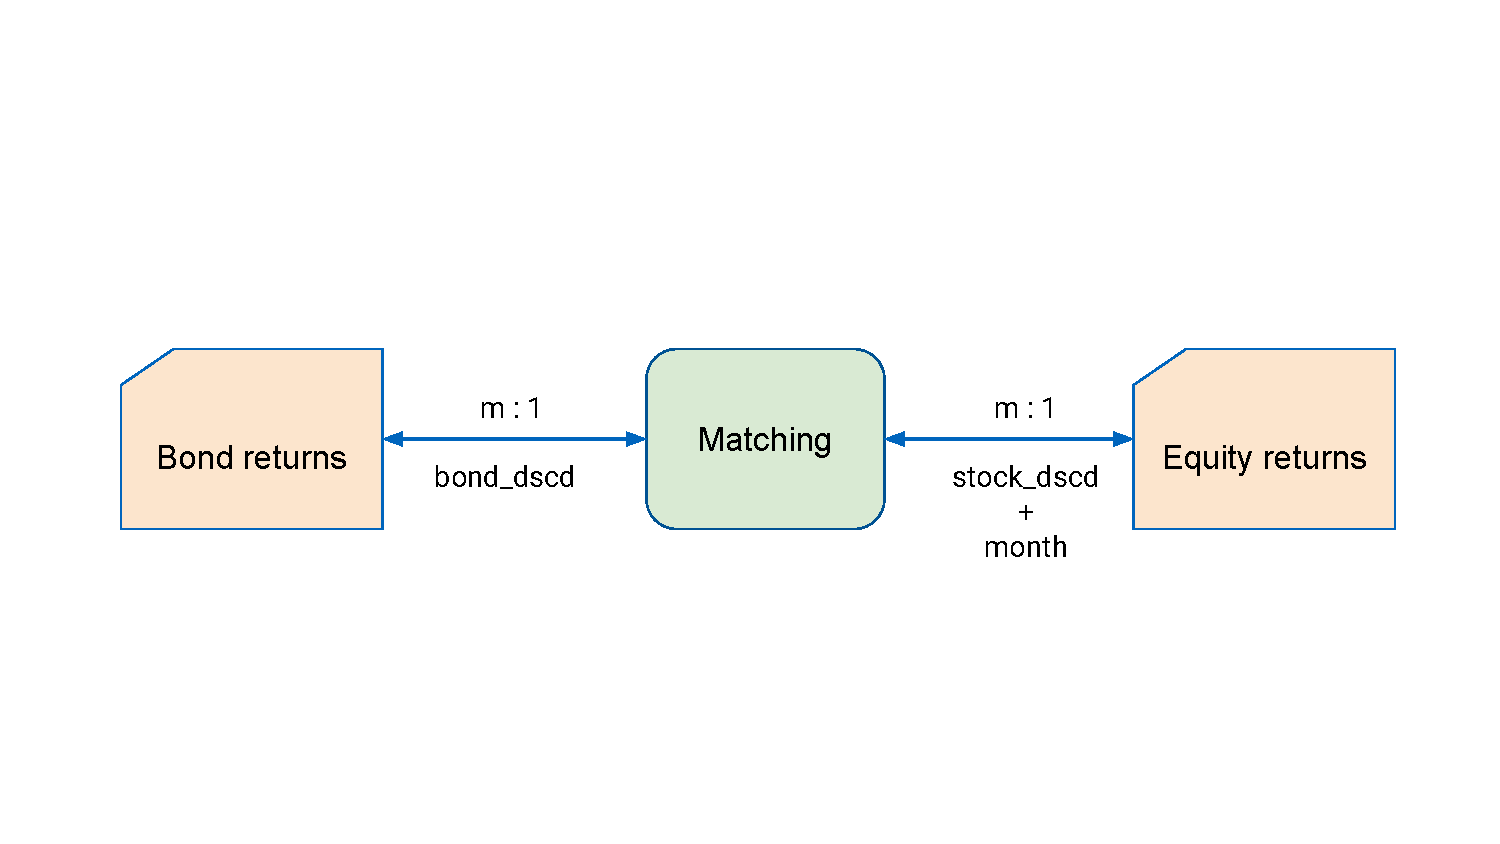
\includegraphics[trim={0 4.5cm 0 5cm},clip,width=1.0\linewidth]{figures/matching-returns.pdf}
	\caption{Matching of Bond and Equity Returns}
	\label{fig:matching-returns}
\end{figure}
After that, the resulting dataset has to be merged with the provided stock time series data, which also includes the required monthly stock returns. This merge should take place over the two parameters $stock\_dscd$ and $month$. This is because we want the bond and stock returns to be comparable for one and the same month later on. When executing the merges in Stata, keep in mind to make sure that the Datastream code parameter is named the same in the bond dataset and the matching (i.e. $bond\_dscd$), and similarly for the stocks and the matching (i.e. $stock\_dscd$). Otherwise, the matching will fail. The bonds-matching merge is performed on a M-to-1 relation, because multiple bonds can be mapped to the same equity over the issuing company. The merge with the equities is performed on a M-to-1 relation as well for the same reason. The resulting database builds the foundation for further statistical analysis. 

\section{Summary Statistics} \label{section:summary-statistics}
Stata offers some very useful tools to determine the underlying distribution of the data, as well as to perform correlation and regression calculations. In order to obtain summary statistics separately for different bond groups, I split the bond returns dataset by geography and by credit rating. 

\begin{figure}[h]
	\centering
	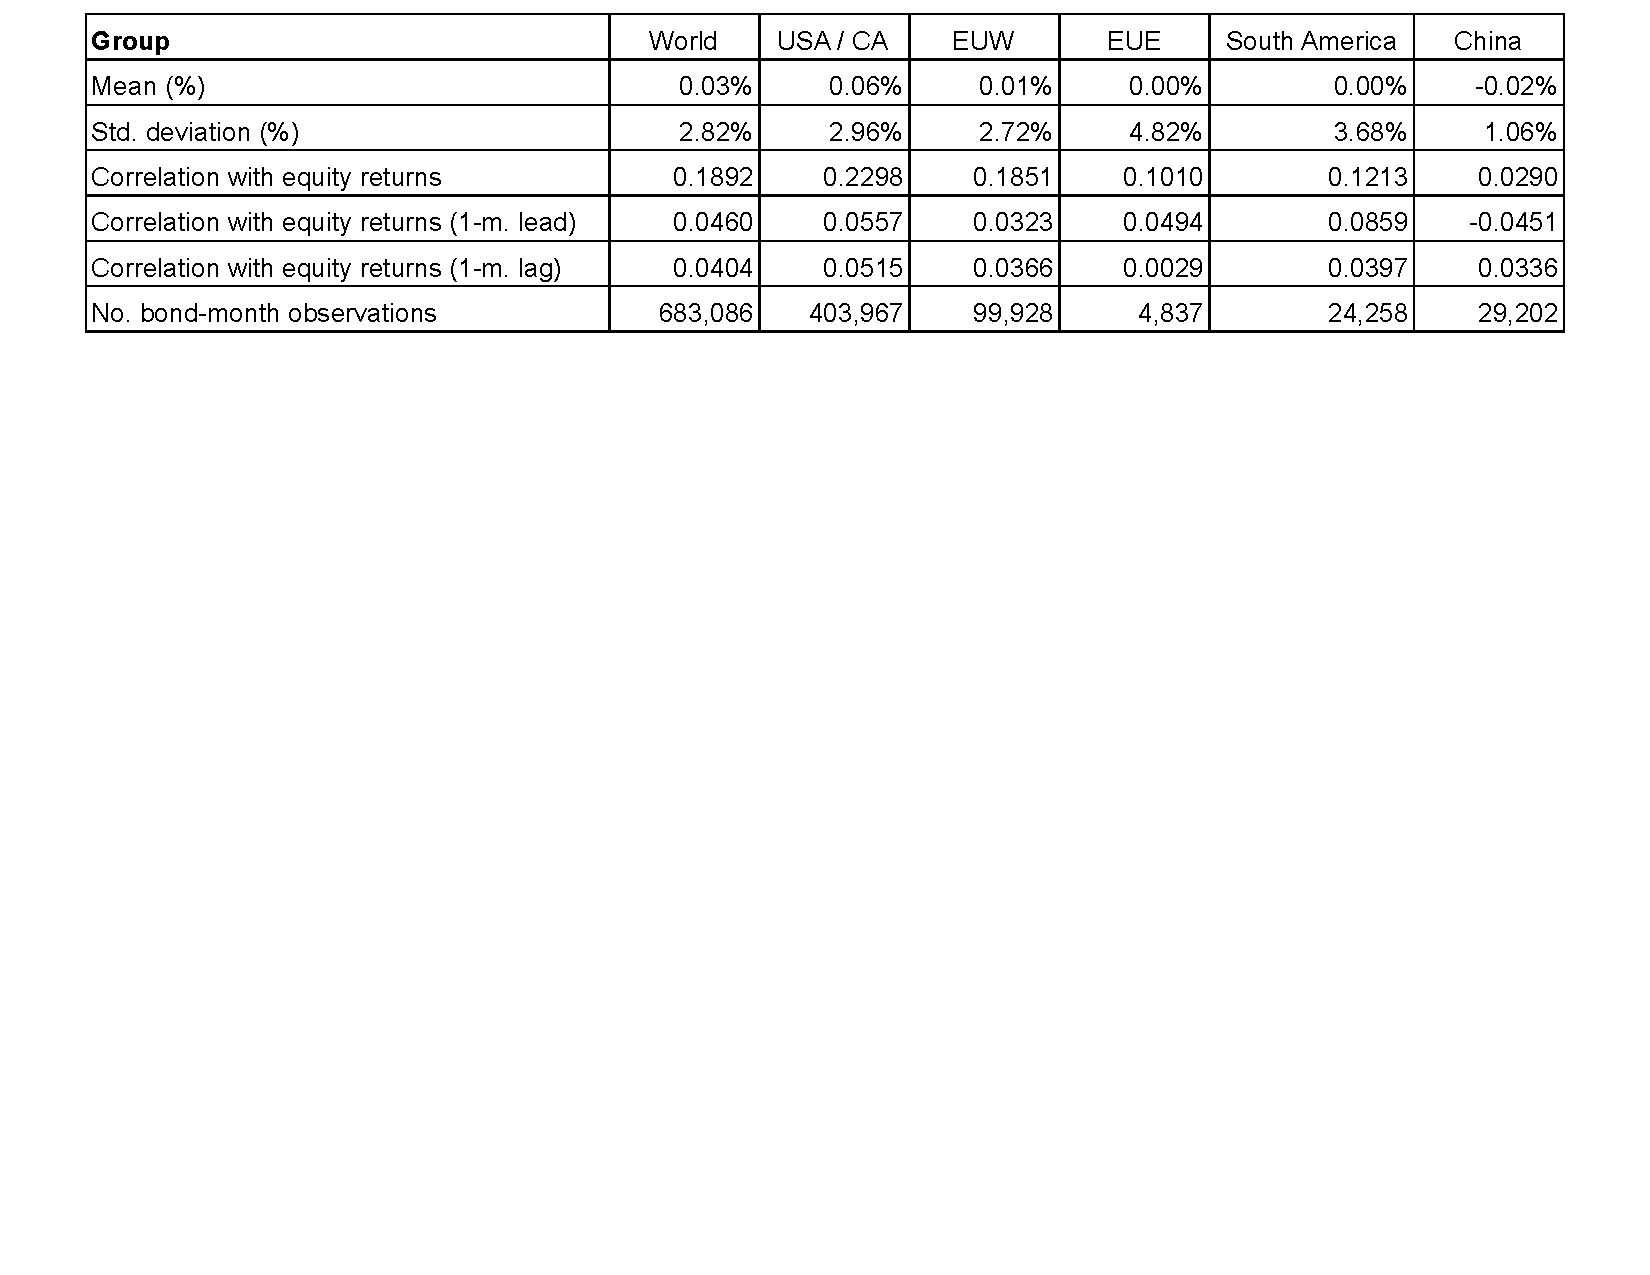
\includegraphics[trim={1cm 15.5cm 1cm 0},clip,width=1.0\linewidth]{figures/summary-stats-by-geo.pdf}
	\caption{Monthly Return Statistics by Bond Geography}
	\label{fig:summary-stats-by-geo}
\end{figure}

Fig. \ref{fig:summary-stats-by-geo} features monthly return statistics for:
\begin{itemize}
	\item The entire world
	\item North America region (NA), represented by USA and Canada
	\item Western Europe region (EUW), represented by Germany, France, UK, Italy, Ireland, Luxembourg, Netherlands, Spain, Portugal, Belgium, Austria, Switzerland, and Scandinavian countries
	\item Eastern Europe region (EUE), represented by Poland, Czech Republic, Bulgaria, Greece, Serbia, Croatia, Hungary, Montenegro, Ukraine, Turkey, and Georgia
	\item South America region, represented by Brazil, Argentina, Chile, Colombia, Uruguay, Paraguay, Panama, Peru, and Mexico (though NA)
	\item China 
\end{itemize}
Note that the list is neither regionally exhaustive, nor is it 100\% geographically accurate. Its sole purpose is to gain a general idea of the distribution of corporate bond returns for countries with a similar financial structure. 

Fig. \ref{fig:summary-stats-by-rating} features monthly return statistics for different credit ratings of corporate bonds. Please note that the number of bond-month observations for the single credit ratings does not sum up to to the number in the \textit{All} column. This is due to the procedure which was used to split the bonds up by their rating. To give an example, bonds listed in rating category \textit{BBB} are those bonds which have either a \textit{BBB} rating as given by the S\&P agency, or a \textit{Baa} rating as given by the Moody's agency. In some cases, it occurs that e.g. the Moody's rating is given as \textit{A}, and the S\&P rating as \textit{BBB}. In this case, the bond would be listed in both the \textit{A} and the \textit{BBB} categories, which results in intersections between the single categories. The procedure has been chosen this way to receive a larger amount of data for analysis, as e.g. entries for the Moody's rating alone were somewhat scarce. If needed, further analysis can be done based on ratings of a single agency only. 

\begin{figure}[h]
	\centering
	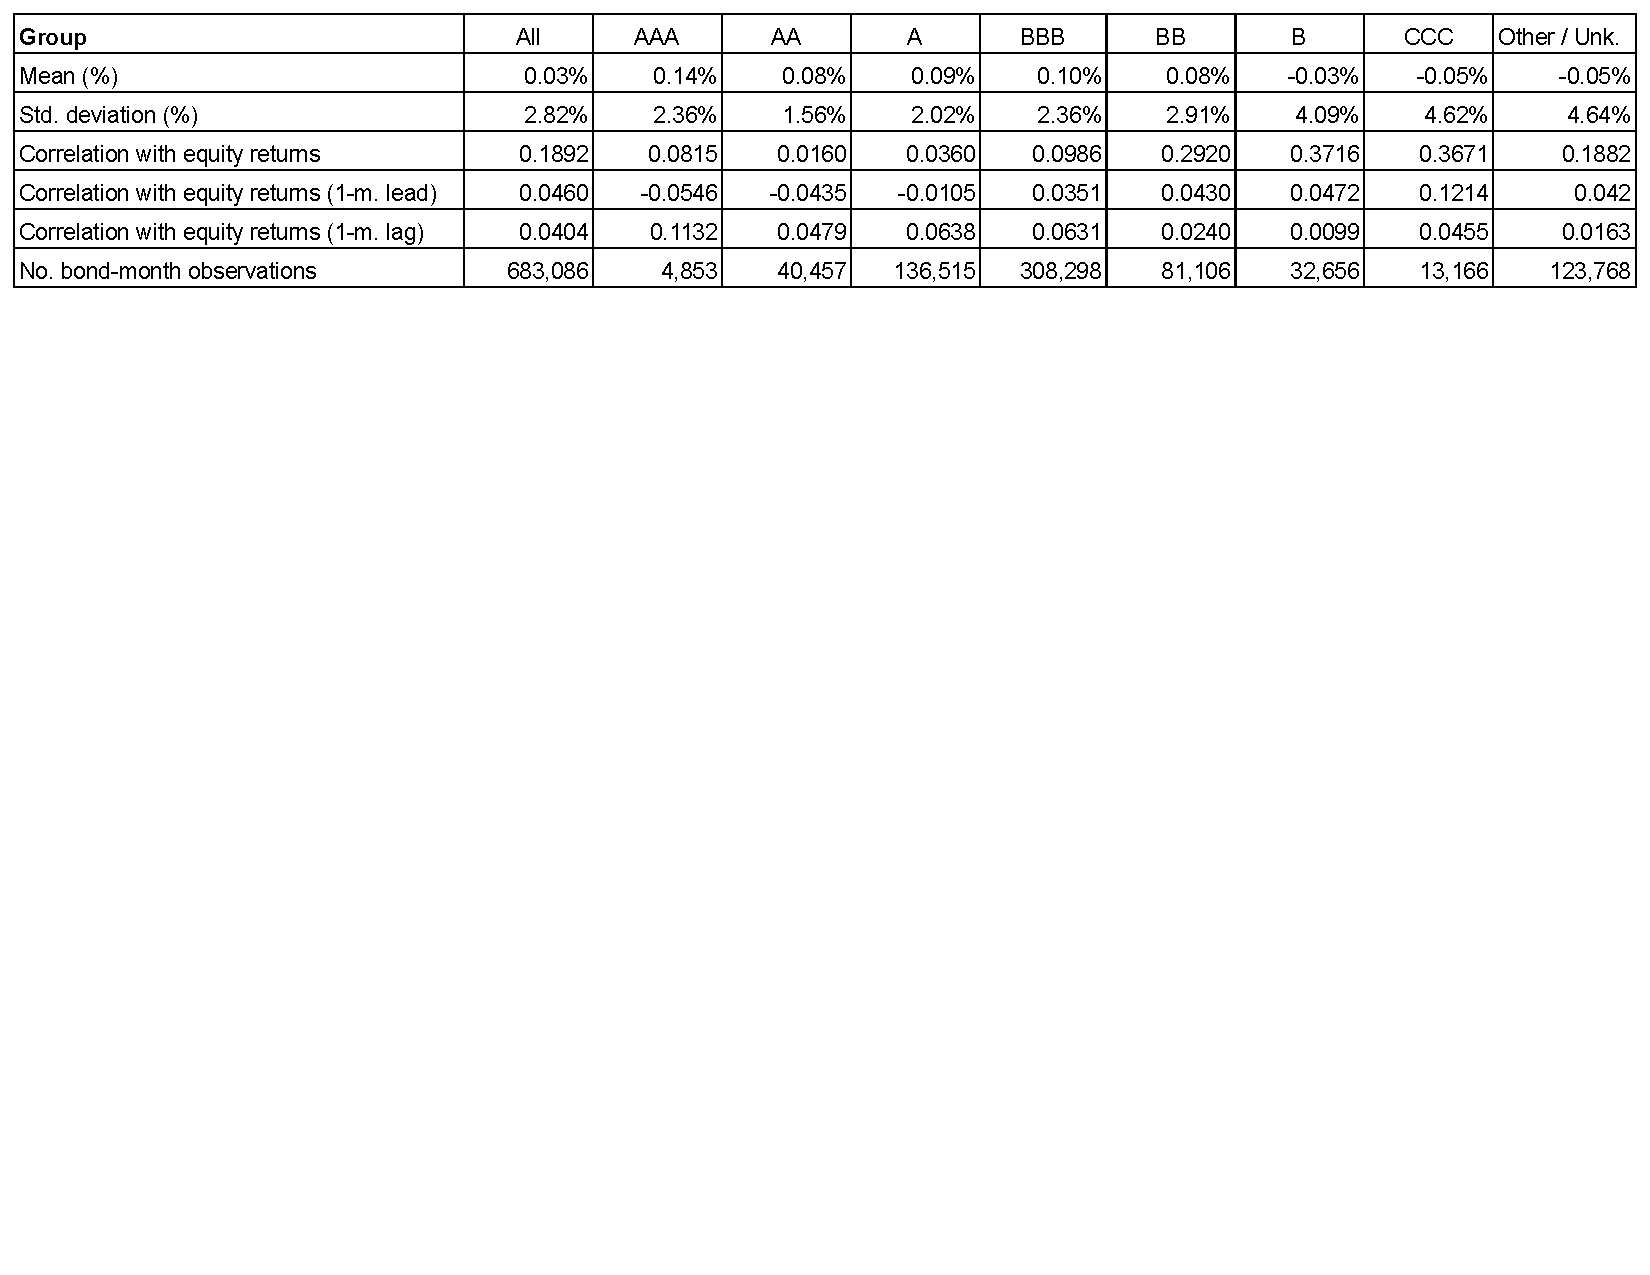
\includegraphics[trim={0 16cm 0 0},clip,width=1.0\linewidth]{figures/summary-stats-by-rating.pdf}
	\caption{Monthly Return Statistics by Bond Rating}
	\label{fig:summary-stats-by-rating}
\end{figure}

The distribution mean and standard deviation of the bond returns are largely in-line with my expectations. Bonds in regions with a majority of developed countries generally have a higher mean return and a lower standard deviation than bonds in regions with more developing countries. Similarly, investment grade bonds have higher mean return and lower volatility than non-investment grade bonds. 

The correlation with equity returns looks higher for developed regions, but at the same time lower for investment grade bonds. 
Additionally, the correlation of monthly bond returns with lagged stock returns strictly monotonically increases with falling credit rating. As such, the lowest bond-lead correlation can be seen for corporate bonds rated \textit{AAA}, while the highest correlation is listed for \textit{CCC} rated bonds. This already explains quite well why existing research on the topic of the lead-lag relation of corporate bonds and stocks mostly focuses on high yield bonds, as these have the highest lead correlation with stocks. The correlation results of stock returns with lagged bond returns are less conclusive, but tend to be higher for investment grade bonds. From a geographical point of view, there seems to be no significant insight for the lead and lag correlations with equity returns. 

\section{Lead-Lag Relationship} \label{section:lead-lag-relationship}
In order to estimate the existence of a potential lead or lag relationship between corporate bonds and stocks, multiple regression analyses have been run. In particular, the calculations were conducted for the following bond groups: 
\begin{itemize}
	\item all corporate bonds
	\item split by geographical region: North America, South America, Western Europe, Eastern Europe, and China
	\item split by bond credit rating: AAA, AA, A, BBB, BB, B, CCC, other
	\item split by aggregated bond credit rating: investment grade and non-investment grade bonds
	\item two rating-based approaches to high-yield bonds
\end{itemize}
All regression analyses have been run as a duo of: 
\begin{enumerate}
	\item regression with monthly bond returns as dependent variable and 1-month lagged stock returns as independent variable
	\item regression with monthly stock returns as dependent variable and 1-month lagged bond returns as independent variable
\end{enumerate}

For shortness, not all the regression results will be introduced here in detail. This section will mostly focus on high yield bonds, as these have shown the most likely lead correlation with equities in section \ref{section:summary-statistics}, and also because the leads and lags of high yield bonds have seen the highest attention in the existing literature on this subject so far (e.g. \cite{lead-lag-source}). All the other regression results can be found either in appendix \ref{appendix-regression} to this work, or as part of the project files. 

\begin{figure}[h]
	\centering
	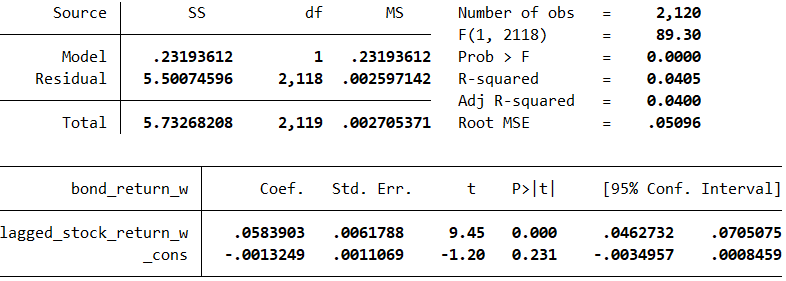
\includegraphics[trim={0 0 0 0},clip,width=1.0\linewidth]{figures/regression-results/regression-high-yield-ccc-d-moodies-bonds-as-dependent.PNG}
	\caption{Results: regression with high-yield corporate bonds (as by Moody's) as dependent variable, and stocks as independent variable}
	\label{fig:regression-high-yield-ccc-d-moodies-bonds-as-dependent.PNG}
\end{figure}

Fig. \ref{fig:regression-high-yield-ccc-d-moodies-bonds-as-dependent.PNG} features the regression results for high-yield corporate bond return as dependent variable, and stock return as independent variable. Specifically, high-yield bonds have been taken as those with either a \textit{Ca} or a \textit{C} current rating provided by Moody's. From a statistical perspective, the following interpretation of the results can be given: 
\begin{itemize}
	\item The \textit{model sum of squares} (\textit{MSS}) is not very close to the \textit{total sum of squares} (\textit{TSS}), which means that the fit of the model function is not very tight. 
	\item The \textit{p-value} (here \textit{Prob $>$ F}) is noticeably lower than 0.05. This means that the results of the regression are statistically significant. 
	\item The $r^2$ is the amount of variance of bond returns that is explained by the lagged equity returns. The number is rather low, though it is the highest achieved in all the regression analyses run. Apparently, equities are best in explaining the variance of high-yield bonds, compared to other bond groups.
	\item The \textit{root mean-squared-error} is the standard deviation of the regression model. It is close to 0, which means that the single bond return values do not deviate much from the distribution mean on average. On the other hand, the bond returns themselves are not very high, so even an absolutely small standard deviation can have a significant impact on the spread. 
	\item The modeled regression function itself has the shape $bond\_return_{n} = -0.0013 + 0.0584 * stock\_return_{n-1}$, with $n$ being the month, at the end of which the return occurred. The magnitude of the steepness factor and the intercept seems in-line with our expectations. 
	\item The \textit{t-values} signify the importance of the variable in the regression model. An absolute \textit{t-value} greater than 1.96 is usually considered as good, which is here the case for the steepness coefficient.  
	\item The \textit{two-tail p-value} (here \textit{P $>$ $|t|$})is lower than 0.05 for the growth coefficient, which means that it is statistically significant. The value for the intercept is not very significant at 0.231. 
\end{itemize}
Overall, the results show that stock returns lead the returns of high yield bonds on a 1-month basis, though the results are not entirely conclusive. My recommendation is to use a more sophisticated (e.g. portfolio-based) regression procedure, and potentially to also try using a non-linear regression model to receive more reliant results. 

\begin{figure}[h]
	\centering
	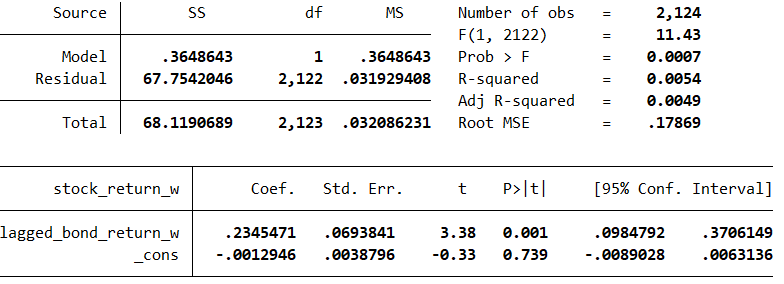
\includegraphics[trim={0 0 0 0},clip,width=1.0\linewidth]{figures/regression-results/regression-high-yield-ccc-d-moodies-stocks-as-dependent.PNG}
	\caption{Results: regression with high-yield corporate bonds (as by Moody's) as independent variable, and stocks as dependent variable}
	\label{fig:regression-high-yield-ccc-d-moodies-stocks-as-dependent.PNG}
\end{figure}

Fig. \ref{fig:regression-high-yield-ccc-d-moodies-stocks-as-dependent.PNG} shows the regression results for high-yield corporate bond return as independent variable, and stock return as dependent variable. The same definition of 'high-yield' applies as for the first regression. Compared to regression results with bonds as dependent variable, the results with stocks as dependent variable are somewhat less significant, as can be seen e.g. by looking at the p-value an the two-tailed p-values. The model function fit is also somewhat worse when looking at the model sum of squares compared to the total sum of squares, as well as based on the $r^2$ parameter and the standard deviation of the model. Based on the t-values and the two-tail p-values, the results are statistically significant for the growth coefficient, but not so for the intercept. The model function itself is shaped as $stock\_return_{n} = -0.0013 + 0.2345 * bond\_return_{n-1}$, with $n$ being the month like before. 

As the results of the second regression model are not as reliable and significant as those of the first one, it can be concluded that stocks are likely faster in incorporating significant market information than high-yield bonds, for one and the same company. However, due to the chosen procedure being very basic, it is advisable to conduct a more thorough regression analysis to draw up more reliable conclusions. 


		\chapter{Conclusion}
\label{chapter:Conclusion}

\section{Summary}
In this work, three of the basic skyline algorithms Naive-Nested-Loops, Block-Nested-Loops and Divide-and-Conquer, as well as the newer ST-S algorithm were introduced. The algorithms were placed into the ``big picture'' of the current state-of-the-art skyline algorithms and explained in detail. Thereafter, the novel skyline algorithm SARTS, which utilizes the highly efficient ART tree, was presented. The algorithm keeps all the advantages of ST-S, while being significantly more memory-efficient at the same time. The algorithms were parallelized using different approaches and frameworks, which were explained in greater detail. In the last chapter, an evaluation of the conducted tests was carried out and the outcomes analyzed. 

With the results of this work, the following points should be considered when choosing the right skyline algorithm for the particular use case: 
\begin{itemize}
	\item When the application scenario assumes continuous attribute values and does not require progressive behavior, then Block-Nested-Loops seems to be a very potent ``all-rounder'' algorithm, well suited for both I/O-intensive as well as in-memory databases. At this point, some of the newer algorithms based on Block-Nested-Loops should be considered, such as SFS~\cite{sfs} and SaLSa~\cite{salsa}. The presorting and the threshold approaches showed that they can improve an algorithm such as ST-S, and thus can be recommended to be applied to BNL as well. 
	\item In a scenario where progressiveness is important, an online-capable algorithm such as ST-S or SARTS should be chosen. Both algorithms perform excellently for medium-range to high $n$ and provide good scalability in parallelized environments. While tree-based algorithms do not scale well with high dimensionality, most online services seem to have a high number of database entries with mostly low dimensionality nowadays\footnote{Consider a database holding around 1 million hotels with 5-10 different categorical attributes each for this purpose.}.
	\item In environments that require efficient memory usage SARTS is highly recommended to be chosen over ST-S due to its significantly lower space consumption. 
\end{itemize}

\section{Outlook}
% parallelization
While the parallelization approaches introduced in this work showed to improve the respective sequential versions of the algorithms, some of them have the potential to perform even better when running on more than 4 threads. This could be further tested, provided that a suiting machine is available. 

% Art baum mit path compression und lazy expansion
The current version of the SARTS algorithm already keeps up with ST-S in terms of computation time, and overtakes it by far in terms of efficient memory usage. Nevertheless, it still can be improved by utilizing not the basic, but the full version of the ART tree, including both lazy expansion and path compression. These techniques enable faster insert operations and dominance checks, and also save even more memory by leaving out unnecessary nodes. It is expected that with these improvements the SARTS algorithm would bypass ST-S both in speed and in efficiency of memory usage. The only (known) successor to ST-S to date is the algorithm TA-SKY, also proposed by the same authors in \cite{rahman}. Thus, it would be interesting to compare an improved version of SARTS to TA-SKY in terms of time and memory management. 

% integration into a DBMS
SARTS was originally developed in the context of an in-memory database, such as HyPer~\cite{hyper}. Still, it also seems suitable for I/O-intensive DBMS due to BNL being one of its ``ancestors''. While performance tests in this work showed that SARTS can deal quite well with synthetic datasets, it is always sensible to test an algorithm on real-world datasets. For this reason, it can be recommended to integrate SARTS in a database system, in order to see how well it fares in this environment. 

% online algorithm
As SARTS should be primarily used as an online algorithm, it also appears sensible to test it within a database system which demands its algorithms to work progressively, i.e. to deliver first results before the entire skyline is computed. Some sort of interactive web application seems fit for this purpose. 
		
%		\part[The 2nd Part]{The Second Part}
%		\label{part:secondP}		
		
		% ---------------------------------------------------------------------------
		%
		% Appendix
		%
		% ---------------------------------------------------------------------------
		
		\part*{Appendix}
		\addcontentsline{toc}{part}{Appendix}
		
		\appendix %---------------------------------------
		
			\chapter{Datastream Extraction Tool Manual} \label{appendix-dset-manual}
\captionsetup{margin=10pt,font=large,labelfont=bf,textfont={bf}}

The full version of the Datastream Extraction Tool Manual can be found in the project folder of the Google Drive repository under \url{https://bit.ly/3rB3lqg}. 

\section{Introduction}
The Datastream Extraction Tool is an application that allows the user to download financial data from Thomson Reuters Datastream without the overhead of doing it manually in Excel. The tool was created specifically for large static and time-series requests, and supports long-duration downloads of data. 

\section{Installation}
Please, be aware of the following: 
\begin{itemize}
	\item The application can only be run on Windows computers. It cannot be ported to MacOS or Linux, as the Thomson Reuters Excel add-in is only available for Windows, and also because the VBA (Visual Basic for Applications) version on Unix-based computers is a different one than on Windows computers. 
	\item While the application can generally be run on remote computers as well, it can be rather inconvenient. On the one hand, remote computers tend to be less stable in terms of internet connection and add-in connectivity. And additionally, the remote computers of TUM-SOM have rather poor performance (especially disk access!), which would constrain the data download. Furthermore, remote computers automatically shut down after some time, which makes downloading large data loads problematic. For smaller requests though, that take up to 1 hour of download time, the remote execution should suffice. 
\end{itemize}

\subsection{Prerequisites}
Please make sure that the following environment is established before you proceed with the installation.
\begin{itemize}
	\item Make sure you have a valid \textbf{Microsoft Office Installation}. The application was tested with Office 365, but it should also run with other recent Office environments.
	\item Make sure that \textbf{Thomson Reuters Eikon \& Datastream} is installed. If you install it for the first time, please ensure that the Datastream add-on in the Excel plug-in is enabled. 
	\item Make sure that you have an up-to-date version of \textbf{Python 3} installed. Python 3 is different from Python 2; with Python 2 the application will not work. 
	\item Make sure that in Windows Power Options you select that your PC "never" goes to sleep. Since otherwise this can interrupt long-running downloads. 
\end{itemize}

\subsection{Download}
Follow these steps to install the application on your computer: 
\begin{enumerate}
	\item Download the \textit{Shippable} folder from \url{https://bit.ly/2VfT058} to your computer. Choose a location with enough free space, as the downloaded data will be stored in-place. 
	\item Unzip the downloaded file. You can rename the root folder from \textit{Shippable} to a different name at your convenience. Please, do \textbf{not} rename any of the folders or files inside. Such changes would need to be propagated to the program code. 
	\item In the \textit{Shippable }folder, you will find a file called \textbf{\textit{prerequisites.py}}. You need to run this file with Python. You can do so by e.g. right-clicking on the file, selecting "Open with" and then choosing Python. It will then automatically install external Python packages needed for the app. 
\end{enumerate}

\subsection{Settings}
Finally, you will need to adjust some settings in Excel the first time you install the application. For this purpose, open the file called \textit{RequestTable.xlsm} in the \textit{Shippabl}e folder. 

The first time you open it, you might get prompted to activate file contents or to allow modifications, etc. Please agree to all such messages. 

Further, take care of the following settings: 
\begin{itemize}
	\item Make sure that both the \textit{Thomson Reuters} tab and the \textit{Thomson Reuters Datastream} tab show in the tab panel of the Excel document. 
	\item In the Thomson Reuters tab go to Settings $=>$ Sign-In $=>$ choose to automatically sign-in whenever Office is started. 
	\item Go to File $ => $ Options $ => $ Trust Center $ => $ Trust Center Settings and do: 
	\begin{itemize}
		\item Macro Settings $ => $ select "\textit{Enable all macros}" and check "\textit{Trust access to the VBA project object model}". 
		\item Protected View $ => $ uncheck all boxes except for "\textit{Outlook attachments}". 
		\item Add-ins $ => $ uncheck all boxes.
		\item External Content $ => $ select "\textit{Enable all Data Connections}", "\textit{Enable automatic update for all Workbook Links}", "\textit{Enable all Linked Data Types}".
	\end{itemize}
	\item Go to File $ => $ Options $ =>  $Customize Ribbon $ => $ select \textit{Main Tabs} on the right $ => $ check the \textit{Developer, Add-ins, Thomson Reuters}, and \textit{Thomson Reuters Datastream} tabs. 
	\item Go to File $ => $ Options $ => $ Advanced $ => $ section \textit{General} $ => $ uncheck option \textit{Ask to update automatic links}. 
	\item Go to File $ => $ Options $ => $ Add-ins and make sure that the add-in \textit{Thomson Reuters Eikon - Microsoft Office }is listed among \textit{Active Application Add-ins}. It should be. If not, refer to the Troubleshooting section. 
	\item Press "Alt + F11" (the VBA editor will appear) $ => $ go to Tools $ => $ References $ => $ check the box near "\textit{Microsoft Scripting Runtime}"
\end{itemize}

Now, you should be well set to run the application.

\section{Usage}
You can start the Datastream Extraction Tool by running the file \textbf{\textit{ds\_extraction\_tool.py}} with Python. 

If you encounter a problem, some other prerequisites on your computer might be missing that might not have been covered in this guide. In that case, please contact the project developer. 


\chapter{C++ Code} \label{appendix-code}
\usemintedstyle{bw}

\section{Dominates Operation for NNL, BNL and DNC}
\begin{minted}[tabsize=3,breaklines,fontsize=\small]{c++}
/**
* Checks whether one tuple dominates the other and returns true|false
* @param dominator the tuple to check for dominating
* @param dominated the tuple to check for being dominated
*/
bool dominates(const std::vector<int> &dominator, const std::vector<int> &dominated){
	bool flag = true;
	for(std::vector<int>::size_type i = 0; i< dominated.size(); i++){
		if(dominator[i] > dominated[i]) return false;
		if(dominated[i] > dominator[i]) flag = false;
	}
	if(flag) return false;
	return true;
}
\end{minted}

\section{Naive-Nested-Loops}
\begin{minted}[tabsize=3,breaklines,fontsize=\small]{c++}
void computeSkylineProduce(){
	for(std::size_t i = 0; i < storage.size(); i++){
		bool not_dominated = true;
		for(std::size_t j = 0; j < storage.size(); j++){
			if(i != j){
				if(dominates(storage[j], storage[i])){
					not_dominated = false;
					break;
				}
			}
		}
		if(not_dominated){
			parent->consume(storage[i]);
		}
	}
}
\end{minted}

\section{Naive-Nested-Loops Parallelized}
\begin{minted}[tabsize=3,breaklines,fontsize=\small]{c++}
void computeSkylineProduceParallel(){
	const std::vector<std::vector<int>> storage = this->storage;
	CatOperator *parent = this->parent;
	parallel_for(std::size_t(0), storage.size(), [this, storage, parent]( std::size_t i ) {
		bool not_dominated = true;
		bool flag = false;
		for(std::size_t j = 0; j < storage.size() && !flag; j++){
			if(i != j){
				if(dominates(storage[j], storage[i])){
					not_dominated = false;
					flag = true;
				}
			}
		}
		// The following mutex slows down the parallelization, but provides an easy way to avoid race conditions
		// In case no mutex is used, the programmer needs to make sure that no race condition occurs in the following if-block
		static spin_mutex mtx;
		spin_mutex::scoped_lock lock(mtx);
		if(not_dominated){
			parent->consume(storage[i]);
		}
	} );
}
\end{minted}

\section{Block-Nested-Loops Volcano Model}
\begin{minted}[tabsize=3,breaklines,fontsize=\small]{c++}
void computeSkyline(){
	// storage is the window here
	storage.push_back(child->getNext());
	while(true){
		std::vector<int> tuple = child->getNext();
		if(!tuple.empty()){
			storage.push_back(tuple);
			for(std::size_t j = 0; j < storage.size()-1; j++){
				if(dominates(storage.back(), storage[j])){
					storage.erase(storage.begin() + j);
					j--;
				}
				else if (dominates(storage[j], storage.back())){
					storage.erase(storage.begin() + storage.size()-1);
					break;
				}
			}
		}
		else break;
	}
}
\end{minted}

\section{Block-Nested-Loops Produce/Consume}
\begin{minted}[tabsize=3,breaklines,fontsize=\small]{c++}
void computeSkylineProduce(){
	// storage contains tuples produced by the generator
	std::vector<std::vector<int>> window;
	window.push_back(storage[0]);
	for(std::size_t i = 1; i < storage.size(); i++){
		std::vector<int> tuple = storage[i];
		window.push_back(tuple);
		for(std::size_t j = 0; j < window.size()-1; j++){
			if(dominates(window.back(), window[j])){
				window.erase(window.begin() + j);
				j--;
			}
			else if (dominates(window[j], window.back())){
				window.erase(window.begin() + window.size()-1);
				break;
			}
		}
	}
	for(std::size_t i = 0; i < window.size(); i++){
		parent->consume(window[i]);
	}
}
\end{minted}

\section{Divide-and-Conquer}

\subsubsection{{\large Algorithm}}
\begin{minted}[tabsize=3,breaklines,fontsize=\small]{c++}
std::vector<std::vector<double>> computeSkyline(const std::vector<std::vector<double>> &M, const int &dimension){
	if(M.size() == 1) return M;
	
	std::vector<double> pivot = median(M, dimension-1); // dimension-1 because we need the last index
	std::pair<std::vector<std::vector<double>>, std::vector<std::vector<double>>> P = partition(M, dimension-1, pivot);
	
	std::vector<std::vector<double>> S_1, S_2;
	S_1 = computeSkyline(P.first, dimension);
	S_2 = computeSkyline(P.second, dimension);
	
	std::vector<std::vector<double>> result;
	std::vector<std::vector<double>> merge_result = mergeBasic(S_1, S_2, dimension);
	
	// Union S_1 and merge_result
	for(std::vector<std::vector<double>>::size_type i = 0; i < S_1.size(); i++){
		result.push_back(S_1[i]);
	}
	for(std::vector<std::vector<double>>::size_type i = 0; i < merge_result.size(); i++){
		result.push_back(merge_result[i]);
	}
	
	return result;
}
\end{minted}

\subsubsection{{\large Partition Operation}}
\begin{minted}[tabsize=3,breaklines,fontsize=\small]{c++}
std::pair<std::vector<std::vector<double>>, std::vector<std::vector<double>>> partition(const std::vector<std::vector<double>> &tuples, const int &dimension, const std::vector<double> &pivot){
	std::vector<std::vector<double>> P_1, P_2;
	std::pair<std::vector<std::vector<double>>, std::vector<std::vector<double>>> partitions;
	
	for(std::vector<std::vector<double>>::size_type i = 0; i < tuples.size(); i++){
		if(tuples[i][dimension] < pivot[dimension])
			P_1.push_back(tuples[i]);
		else
			P_2.push_back(tuples[i]);
	}
	
	partitions.first = P_1;
	partitions.second = P_2;
	
	return partitions;
}
\end{minted}
\subsubsection{{\large Merge Operation}}
\begin{minted}[tabsize=3,breaklines,fontsize=\small]{c++}
std::vector<std::vector<double>> mergeBasic(std::vector<std::vector<double>> S_1, const std::vector<std::vector<double>> &S_2, const int &dimension){
	std::vector<std::vector<double>> result;
	
	if(S_2.size() == 0) return result;
	
	if(S_1.size() == 1){ // trivial case - S_1 has only 1 tuple
		for(std::vector<std::vector<double>>::size_type i = 0; i < S_2.size(); i++){
			if(!dominates(S_1[0], S_2[i]))
				result.push_back(S_2[i]);
		}
	}
	else if(S_2.size() == 1){ // trivial case - S_2 has only 1 tuple
		result.push_back(S_2[0]);
		for(std::vector<std::vector<double>>::size_type i = 0; i < S_1.size(); i++){
			if(dominates(S_1[i], S_2[0])){
				result.erase(result.begin());
				break;
			}
		}
	}
	else if(S_1[0].size() == 2){ // low dimension
		// Min from S_1 according to dimension 1
		std::sort(S_1.begin(), S_1.end(), [](const std::vector<double> &a, const std::vector<double> &b){
			return a[0] < b[0];
		});
		std::vector<double> min = S_1[0];
		// Compare S_2 to Min according to dimension 1; in dimension 2 S_1 is always better
		for(std::vector<std::vector<double>>::size_type i = 0; i < S_2.size(); i++){
			if(S_2[i][0] < min[0]) result.push_back(S_2[i]);
		}
	}
	else{ // general case
		std::vector<double> pivot = median(S_1, dimension-1-1);
		std::pair<std::vector<std::vector<double>>, std::vector<std::vector<double>>> partitions_dim_1 = partition(S_1, dimension-1-1, pivot);
		std::pair<std::vector<std::vector<double>>, std::vector<std::vector<double>>> partitions_dim_2 = partition(S_2, dimension-1-1, pivot);
		std::vector<std::vector<double>> result_1, result_2, result_3;
		
		result_1 = mergeBasic(partitions_dim_1.first, partitions_dim_2.first, dimension);
		result_2 = mergeBasic(partitions_dim_1.second, partitions_dim_2.second, dimension);
		result_3 = mergeBasic(partitions_dim_1.first, result_2, dimension-1);
		
		// Union result_1 and result_3
		for(std::vector<std::vector<double>>::size_type i = 0; i < result_1.size(); i++){
			result.push_back(result_1[i]);
		}
		for(std::vector<std::vector<double>>::size_type i = 0; i < result_3.size(); i++){
			result.push_back(result_3[i]);
		}
	}
	
	return result;
}
\end{minted}

\section{ST-S/ SARTS}
\begin{minted}[tabsize=3,breaklines,fontsize=\small]{c++}
void computeSkylineProduce(){
	// pre-sort tuples in place
	sort(storage);
	std::vector<int> t_stop = storage[0];
	tree.insert(storage[0], tree.root, 0);
	parent->consume(storage[0]);
	for(std::size_t i = 1; i < storage.size(); i++){
		// stop if all the tuples left are dominated à-priori
		if((max(t_stop) <= min(storage[i])) && (t_stop != storage[i])){
			return;
		}
		// check for dominance
		if(!tree.is_dominated(storage[i], tree.root, 0, tree.score(storage[i]))){
			parent->consume(storage[i]);
			tree.insert(storage[i], tree.root, 0);
			if(max(storage[i]) < max(t_stop)){
				t_stop = storage[i];
			}
		}
	}
}
\end{minted}

\section{ST-S/ SARTS Parallelized}

\subsubsection{{\large Algorithm}}
\begin{minted}[tabsize=3,breaklines,fontsize=\small]{c++}
void computeSkylineProduce(){
	const std::vector<std::vector<int>> storage = this->storage;
	const std::size_t number_of_threads = NUMBER_OF_THREADS;
	std::vector<Tree*> subtrees;
	for(std::size_t i = 0; i < NUMBER_OF_THREADS; i++){
		Tree* subtree = new Tree(tree.get_attributes());
		subtrees.push_back(subtree);
	}
	std::future<void> futures[NUMBER_OF_THREADS];	
	// compute subquery skylines
	for(std::size_t i = 0; i < number_of_threads; i++){
		std::vector<std::vector<int>> subset;
		if(i == number_of_threads-1){
			subset.resize(storage.size() / number_of_threads + storage.size() % number_of_threads);
		}
		else{
			subset.resize(storage.size() / number_of_threads);
		}
		for(std::size_t j = 0; j < subset.size(); j++){
			subset[j] = storage[i*(storage.size()/number_of_threads) + j];
		}
		// Replace &ParallelSTS by &ParallelSARTS to receive SARTS
		futures[i] = std::async(std::launch::async, &ParallelSTS::computeSkylineSubset, this, i, subset, subtrees[i]);
	}
	for(std::size_t i = 0; i < NUMBER_OF_THREADS; i++){
		futures[i].get();
	}	
	// compute final skyline
	std::vector<std::vector<int>> input;
	for(std::size_t i = 0; i < subset_results.size(); i++){
		if(!subset_results[i].empty()){
			input.push_back(subset_results[i]);
		}
	}
	sort(input);
	std::vector<int> t_stop = input[0];
	tree.insert(input[0], tree.root, 0);
	parent->consume(input[0]);
	for(std::size_t i = 1; i < input.size(); i++){
		if((max(t_stop) <= min(input[i])) && (t_stop != input[i])){
			return;
		}
		if(!ntree.is_dominated(input[i], tree.root, 0, tree.score(input[i]))){
			parent->consume(input[i]);
			tree.insert(input[i], tree.root, 0);
			if(max(input[i]) < max(t_stop)){
				t_stop = input[i];
			}
		}
	}
	// free memory
	for(std::size_t i = 0; i < subtrees.size(); i++){
		if(subtrees[i] != nullptr) delete subtrees[i];
	}
}
\end{minted}
\subsubsection{{\large ComputeSkylineSubset Operation}}
\begin{minted}[tabsize=3,breaklines,fontsize=\small]{c++}
void computeSkylineSubset(unsigned threadNumber, std::vector<std::vector<int>> tuples, Tree* tree){
	// pre-sort tuples in place
	sort(tuples);
	std::vector<int> t_stop = tuples[0];
	tree->insert(tuples[0], tree->root, 0);
	subset_results[threadNumber * (subset_results.size() / NUMBER_OF_THREADS) + 0] = tuples[0];
	for(std::size_t k = 1; k < tuples.size(); k++){
		// stop if all tuples left are dominated a-priori
		if((max(t_stop) <= min(tuples[k])) && (t_stop != tuples[k])){
			return;
		}
		// check for dominance
		if(!tree->is_dominated(tuples[k], tree->root, 0, tree->score(tuples[k]))){
			subset_results[threadNumber * (subset_results.size() / NUMBER_OF_THREADS) + k] = tuples[k];
			tree->insert(tuples[k], tree->root, 0);
			if(max(tuples[k]) < max(t_stop)){
				t_stop = tuples[k];
			}
		}
	}
}
\end{minted}

\section{N-Tree}

\subsubsection{{\large Insert Operation}}
\begin{minted}[tabsize=3,breaklines,fontsize=\small]{c++}
void NTree::insert(const std::vector<int> &tuple, node* p, unsigned int level){
	if(level == 0){
		p->minScore = 0;
		p->maxScore = 0;
		for(std::size_t i = 0; i < tuple.size(); i++){
			p->maxScore += (int) (pow(2.0, (double) (tuple.size()-i)) * attributes[attributes.size()-1]);
		}
	}
	else{
		p->minScore = 0;
		for(std::size_t i = 0; i < level; i++){
			p->minScore += (int) (pow(2.0, (double) (tuple.size()-i)) * tuple[i]);
		}
		p->maxScore = p->minScore;
		for(std::size_t i = level; i < tuple.size(); i++){
			p->maxScore += (int) (pow(2.0, (double) (tuple.size()-i)) * attributes[attributes.size()-1]);
		}
	}
	if(level == tuple.size()){
		p->tupleIDs.push_back(tupleID++);
	}
	else{
		if(p->children.empty()){
			p->children.resize(attributes.size());
		}
		if(!p->children[tuple[level]]){
			p->children[tuple[level]]=new node();
		}
		insert(tuple, p->children[tuple[level]], level+1);
	}
}
\end{minted}

\subsubsection{{\large Is\_Dominated Operation}}
\begin{minted}[tabsize=3,breaklines,fontsize=\small]{c++}
bool NTree::is_dominated(const std::vector<int> &tuple, node* p, unsigned int level, unsigned int currentScore){
	if(p==nullptr || (currentScore < p->minScore)){
		return false;
	}
	if((level == tuple.size()) && (score(tuple) != p->minScore)){
		return true;
	}
	if((level == tuple.size()) && (score(tuple) == p->minScore)){
		return false;
	}
	// search the subtrees from left to right
	unsigned int weight = (int) (pow(2.0, (double) (tuple.size()-level)) * tuple[level]);
	for(int i = 0; i < tuple[level]; i++){
		if(is_dominated(tuple, p->children[i], level+1, currentScore + weight)){
			return true;
		}
	}
	if(is_dominated(tuple, p->children[tuple[level]], level+1, currentScore)){
		return true;
	}
	return false;
}
\end{minted}

\section{ART}
%\subsection{Nodes}

\subsubsection{{\large Insert Operation}}
\begin{minted}[tabsize=3,breaklines,fontsize=\small]{c++}
void ART::insert(const std::vector<int> &tuple, Node *&parent, Node *&current, unsigned int level){
	if(level == 0){
		current->minScore = 0;
		current->maxScore = 0;
		for(std::size_t i = 0; i < tuple.size(); i++){
			current->maxScore += (int) (pow(2.0, (double) (tuple.size()-i)) * attributes[attributes.size()-1]);
		}
	}
	else{
		current->minScore = 0;
		for(std::size_t i = 0; i < level; i++){
			current->minScore += (int) (pow(2.0, (double) (tuple.size()-i)) * tuple[i]);
		}
		current->maxScore = current->minScore;
		for(std::size_t i = level; i < tuple.size(); i++){
			current->maxScore += (int) (pow(2.0, (double) (tuple.size()-i)) * attributes[attributes.size()-1]);
		}
	}
	if(level == tuple.size()){
		current->tupleIDs.push_back(tupleID++);
	}
	else{
		Node* child = findChild(current, tuple[level]);
		if(!child){
			switch(current->type){
				case NodeType4:
					if(current->count == 4) 
						grow(parent, current, tuple[level-1]);
					break;
				case NodeType16:
					if(current->count == 16) 
						grow(parent, current, tuple[level-1]);
					break;
				case NodeType48:
					if(current->count == 48) 
						grow(parent, current, tuple[level-1]);
					break;
				case NodeType256:
				default:
					break;
			}
			child = newChild(current, tuple[level]);
		}
		insert(tuple, current, child, level+1);
	}
}
\end{minted}

\subsubsection{{\large Is\_Dominated Operation}}
\begin{minted}[tabsize=3,breaklines,fontsize=\small]{c++}
bool ART::is_dominated(const std::vector<int> &tuple, Node* p, unsigned int level, unsigned int currentScore){
	if(p==NULL || (currentScore < p->minScore)){
		return false;
	}
	if((level == tuple.size()) && (score(tuple) != p->minScore)){
		return true;
	}
	if((level == tuple.size()) && (score(tuple) == p->minScore)){
		return false;
	}
	// search the subtrees from left to right
	unsigned int weight = (int) (pow(2.0, (double) (tuple.size()-level)) * tuple[level]);
	for(int i = 0; i < tuple[level]; i++){
		Node* child = findChild(p, i);
		if(child){ // if child not null
			if(is_dominated(tuple, child, level+1, currentScore + weight)){
				return true;
			}
		}
	}
	Node* child = findChild(p, tuple[level]);
	if(child){
		if(is_dominated(tuple, child, level+1, currentScore)){
			return true;
		}
	}
	return false;
}
\end{minted}

\subsubsection{{\large Find\_Child Operation}}
\begin{minted}[tabsize=3,breaklines,fontsize=\small]{c++}
Node* ART::findChild(Node* parent, const int &attribute){
	switch(parent->type){
		case NodeType4: {
			Node4* node = static_cast<Node4*>(parent);
			for (unsigned i = 0; i < node->count; i++){
				if (node->key[i] == attribute){
					return node->children[i];
				}
			}
			return NULL;
		}
		case NodeType16: {
			Node16* node = static_cast<Node16*>(parent);
			for (unsigned i = 0; i < node->count; i++){
				if (node->key[i] == attribute){
					return node->children[i];
				}
			}
			return NULL;
		}
		case NodeType48: {
			Node48* node = static_cast<Node48*>(parent);
			if (node->childIndex[attribute] != emptyMarker){
				return node->children[node->childIndex[attribute]];
			}
			else
				return NULL;
		}
		case NodeType256: {
			Node256* node = static_cast<Node256*>(parent);
			return node->children[attribute];
		}
		default: {
			return NULL;
		}
	}
}
\end{minted}

\subsubsection{{\large New\_Child Operation}}
\begin{minted}[tabsize=3,breaklines,fontsize=\small]{c++}
Node* ART::newChild(Node *&node, const int &attribute){
	Node4* child = new Node4();
	switch(node->type){
		case NodeType4: {
			Node4* parent = static_cast<Node4*>(node);
			unsigned pos;
			// make free space for the new child entry
			for (pos = 0; (pos < parent->count) && (parent->key[pos] < attribute); pos++);
			memmove(parent->key+pos+1, parent->key+pos, parent->count-pos);
			memmove(parent->children+pos+1, parent->children+pos, (parent->count-pos)*sizeof(Node*));
			parent->key[pos] = attribute;
			parent->children[pos] = child;
			parent->count++;
			break;
		}
		case NodeType16: {
			Node16* parent = static_cast<Node16*>(node);
			unsigned pos;
			// make free space for the new child entry
			for (pos = 0; (pos < parent->count) && (parent->key[pos] < attribute); pos++);
			memmove(parent->key+pos+1, parent->key+pos, parent->count-pos);
			memmove(parent->children+pos+1, parent->children+pos, (parent->count-pos)*sizeof(Node*));
			parent->key[pos] = attribute;
			parent->children[pos] = child;
			parent->count++;
			break;
		}
		case NodeType48: {
			Node48* parent = static_cast<Node48*>(node);
			unsigned pos = parent->count;
			// if there are empty slots inbetween, use them instead of appending the child pointer at the end
			if(parent->children[pos]){
				for(pos = 0; parent->children[pos] != NULL; pos++);
			}
			parent->children[pos] = child;
			parent->childIndex[attribute] = pos;
			parent->count++;
			break;
		}
		case NodeType256: {
			Node256* parent = static_cast<Node256*>(node);
			parent->children[attribute] = child;
			parent->count++;
			break;
		}
		default:
			break;
	}
	return child;
}
\end{minted}

\subsubsection{{\large Grow Operation}}
\begin{minted}[tabsize=3,breaklines,fontsize=\small]{c++}
void ART::grow(Node *&parent, Node *&node, const int &indexOfCurrent){
	Node* newNode;
	switch(node->type){
		case NodeType4:
			newNode = new Node16();
			newNode->count = 4;
			for(std::size_t i = 0; i < 4; i++){
				static_cast<Node16*>(newNode)->key[i] = static_cast<Node4*>(node)->key[i];
			}
			for(std::size_t i = 0; i < 4; i++){
				static_cast<Node16*>(newNode)->children[i] = static_cast<Node4*>(node)->children[i];
			}
			break;
		case NodeType16:
			newNode = new Node48();
			newNode->count = 16;
			for(std::size_t i = 0; i < 16; i++){
				static_cast<Node48*>(newNode)->children[i] = static_cast<Node16*>(node)->children[i];
			}
			for (unsigned i = 0; i < node->count; i++){
				static_cast<Node48*>(newNode)->childIndex [static_cast<Node16*>(node)->key[i]] = i;
			}
			break;
		case NodeType48:
			newNode = new Node256();
			newNode->count = 48;
			for (unsigned i = 0; i < 256; i++){
				if (static_cast<Node48*>(node)->childIndex[i] != 48){ // slot not empty
					static_cast<Node256*>(newNode)->children[i] = static_cast<Node48*>(node)->children [static_cast<Node48*>(node)->childIndex[i]];
				}
			}
			break;
		default:
			break;
	}
	newNode->minScore = node->minScore;
	newNode->maxScore = node->maxScore;
	for(std::size_t i = 0; i < node->tupleIDs.size(); i++){
		newNode->tupleIDs[i] = node->tupleIDs[i];
	}
	
	if(node != root){
		// Code to updateParent() is not given for space reasons. Contact the author if needed. 
		updateParent(parent, newNode, indexOfCurrent);
	}
	delete node;
	node = newNode;
}
\end{minted}







	


  \clearemptydoublepage
  
  \bibliography{bibliography/literature}
	
 
\end{document}

